\setcounter{chapter}{5}

\chapter{Interpreting Regression Results}

{\small \textit{Chapter Preview}. A regression analyst collects
data, selects a model and then reports on the findings of the study,
in that order. This chapter considers these three topics in
\emph{reverse} order, emphasizing how each stage of the study is
influenced by preceding steps. An application, determining a firm's
characteristics that influence its effectiveness in managing risk,
illustrates the regression modeling process from start to finish.}

\bigskip

\bigskip


Studying a problem using a regression modeling process involves a
substantial commitment of time and energy. One must first embrace
the concept of \emph{statistical thinking}, a willingness to use
data actively as part of a decision making process. Second, one must
appreciate the usefulness of a model that is used to approximate a
real situation. Having made this substantial commitment, there is a
natural tendency to ``oversell'' the results of statistical methods
such as regression analysis. By overselling any set of ideas,
consumers eventually become disappointed when the results do not
live up to their expectations. This chapter begins in Section 6.1 by
summarizing what we can reasonably expect to learn from regression
modeling.

\marginparjed{``All models are wrong, but some are useful.'' (Box,
1979)}

Models are designed to be much simpler than relationships among
entities that exist in the real world. A model is merely an
approximation of reality. As stated by George Box (1979), ``All
models are wrong, but some are useful.'' Developing the model, the
subject of Chapter 5, is part of the art of statistics. Although the
principles of variable selection are widely accepted, the
application of these principles can vary considerably among
analysts. The resulting product has certain aesthetic values and is
by no means predetermined. Statistics can be thought of as the art
of reasoning with data. Section 6.2 will underscore the importance
of variable selection.

Model formulation and data collection form the first stage of the
modeling process. Students of statistics are usually surprised at
the difficulty of relating ideas about relationships to available
data. These difficulties include a lack of readily available data
and the need to use certain data as proxies for ideal information
that is not available numerically. Section 6.3 will describe several
types of difficulties that can arise when collecting data. Section
6.4 will describe some models to alleviate these difficulties.

\section{What the Modeling Process Tells Us}

Model inference is the final stage of the modeling process. By
studying the behavior of models, we hope to learn something about
the real world. Models serve to impose an order on reality and
provide a basis for understanding reality through the nature of the
imposed order. Further, statistical models are based on reasoning
with the available data from a sample. Thus, models serve as an
important guide for predicting the behavior of observations outside
the available sample.

\subsection{Interpreting Individual Effects}

When interpreting results from multiple regression, the main goal is
often to convey the importance of individual variables, or effects,
on an outcome of interest. The interpretation depends on whether or
not the effects are substantively significant, statistically
significant and causal.

\index{significance!substantive}

\noindent \textbf{Substantive Significance}. Readers of a regression
study first want to understand the direction and magnitude of
individual effects. Do females have more or less claims than males
in a study of insurance claims? If less, by how much? You can give
answers to these questions through a table of regression
coefficients. Moreover, to give a sense of the reliability of the
estimates, you may also wish to include the standard error or a
confidence interval, as introduced in Section 3.4.2.

Recall that regression coefficients are estimates of partial
derivatives of the regression function
\begin{equation*}
\mathrm{E~}y = \beta_0 + \beta_1 x_1 +...+\beta _k x_k.
\end{equation*}
When interpreting coefficients for continuous explanatory variables,
it is helpful to do so in terms of meaningful changes of each $x$.
For example, if population is an explanatory variable, we may talk
about the expected change in $y$ per 1,000 or one million change in
population. Moreover, when interpreting regression coefficients,
comment on their ``substantive'' significance. For example, suppose
that we find a difference in claims between males and females but
the estimated difference is only 1\% of expected claims. This
difference may well be statistically significant but not
economically meaningful. Substantive significance refers to
importance in the field of inquiry; in actuarial science, this is
typically financial or economic significance but could also be
non-monetary, such as effects on future life expectancy.

\marginparjed{Substantive significance refers to importance in the
field of inquiry.}

\index{significance!statistical}

\noindent \textbf{Statistical Significance}. Are the effects due to
chance? The hypothesis testing machinery introduced in Section 3.4.1
provides a formal mechanism for answering this question. Tests of
hypotheses are useful in that they provide a formal, agreed-upon
standard, for deciding whether or not a variable provides an
important contribution to an expected response. When interpreting
results, typically researchers cite a $t$-ratio or a $p$-value to
demonstrate statistical significance.

In some situations, it is of interest to comment on variables that
are \emph{not} statistically significant. Effects that are not
statistically significant have standard errors that are large
relative to the regression coefficients. In Section 5.5.2, we
expressed this standard error as
\begin{equation}\label{E6:StdErrorBeta}
se(b_{j})=s\frac{\sqrt{VIF_{j}}}{s_{x_{j}}\sqrt{n-1}}.
\end{equation}
One possible explanation for a lack of statistical significance is a
large variation in the disturbance term. By expressing the standard
error in this form, we see that the larger the natural variation, as
measured by $s$, the more difficult it is to reject the null
hypothesis of no effect ($H_0$), other things being equal.

A second possible explanation for the lack of statistical
significant is the high collinearity, as measured by $VIF_j$. A
variable may be be confounded with other variables such that, from
the data being analyzed, it is impossible to distinguish the effects
of one variable from another.

A third possible explanation is the sample size. Suppose that a
mechanism similar to draws from a stable population is used to
observe the explanatory variables. Then, the standard deviation of
$x_j,s_{x_j},$ should be stable as the number of draws increases.
Similarly, so should $R_j^2$ and $s^2$. Then, the standard error
$se(b_j)$ should decrease as the sample size, $n$, increases.
Conversely, a smaller sample size means a larger standard error,
other things being equal. This means that we may not be able to
detect the importance of variables in small or moderate size
samples.

Thus, in an ideal world, if you do not detect statistical
significance where it was hypothesized (and fully expected), you
could: (i) get a more precise measure of $y$, thus reducing its
natural variability, (ii) re-design the sample collection scheme so
that the relevant explanatory variables are less redundant and (iii)
collect more data. Typically, these options are not available with
observational data but it can nonetheless be helpful to point out
the next steps in a research program.


\marginparjed{Large samples provide an opportunity to detect the
importance of variables that might go unnoticed in small samples.}

Analysts occasionally observe statistically significant
relationships that were not anticipated - these could be due to a
large sample size. Above we noted that a small sample may not
provide enough information to detect meaningful relationships. The
flip side of this argument is that, for large samples, we have an
opportunity for detecting the importance of variables that might go
unnoticed in small or even moderate size samples. Unfortunately, it
also means that variables with small parameter coefficients, that
contribute little to understanding the variation in the response,
can be judged to be significant using our decision-making
procedures. This serves to highlight the difference between
substantive and statistical significance - particularly for large
samples, investigators encounter variables that are
\textit{statistically significant but practically unimportant}. In
these cases, it can be prudent for the investigator to omit
variables from the model specification when their presence is not in
accord with accepted theory, even if they are judged statistically
significant.

\marginparjed{Variables can be statistically significant but
practically unimportant.}

\index{significance!causal effect}

\noindent \textbf{Causal Effects}. If we change $x$, would $y$
change? As students of basic sciences, we learned principles
involving actions and reactions. Adding mass to a ball in motion
increases the force of its impact into a wall. However, in the
social sciences, relationships are probabilistic, not deterministic,
and hence more subtle. For example, as age ($x$) increases, the
one-year probability of death ($y$) increases for most human
mortality curves. Understanding causality, even probabilistic, is
the root of all science and provides the basis for informed
decision-making.

It is important to acknowledge that causal processes generally
cannot be demonstrated exclusively from the data; the data can only
present relevant empirical evidence serving as a link in a chain of
reasoning about causal mechanisms. For causality, there are three
necessary conditions: (i) statistical association between variables,
(ii) appropriate time order and (iii) the elimination of alternative
hypotheses or establishment of a formal causal mechanism.

As an example, recall the Section 1.1 Galton study, relating adult
children's height ($y$) to an index of parents' height ($x$). For
this study, it was clear that there is a strong statistical
association between $x$ and $y$. The demographics also make it clear
that the parents measurements ($x$) precedes the children
measurements ($y$). What is uncertain is the causal mechanism. For
example, in Section 1.5, we cited the possibility that an omitted
variable, family diet, could be influencing both $x$ and $y$.
Evidence and theories from human biology and genetics are needed to
establish a formal causal mechanism.

\linejed\index{examples!race, redlining and automobile insurance
prices}\index{actuarial \& financial terms and concepts!redlining}

\textbf{Example: Race, Redlining and Automobile Insurance Prices.}
In an article with this title, Harrington and Niehaus (1998)
investigated whether insurance companies engaged in (racial)
discriminatory behavior, often known as \emph{redlining}. Racial
discrimination is illegal and insurance companies may not use race
in determining prices. The term redlining refers to the practice of
drawing red lines on a map to indicate areas that insurers will not
serve, areas typically containing a high proportion of minorities.

To investigate whether or not there exists racial discrimination in
insurance pricing, Harrington and Niehaus gathered private passenger
premiums and claims data from the Missouri Department of Insurance
for the period 1988-1992. Although insurance companies do not keep
race/ethnicity information in their premiums and claims data, such
information is available at the zip code level from the US Census
Bureau. By aggregating premiums and claims up to the zip code level,
Harrington and Niehaus were able to assess whether areas with a
higher percentage of blacks paid more for insurance (PCTBLACK).

A widely used pricing measure is the loss ratio, defined to be the
ratio of claims to premiums. This measures insurers' profitably; if
racial discrimination exists in pricing, one would expect to see a
low loss ratio in areas with a high proportion of minorities.
Harrington and Niehaus used this as the dependent variable, after
taking logarithms to address the skewness in the loss ratio
distribution.

Harrington and Niehaus (1998) studied 270 zip codes surrounding six
major cities in Missouri where there were large concentrations of
minorities. Table \ref{T6:LossRatio} reports findings from
comprehensive coverage although the authors also investigated
collision and liability coverage. In addition to the primary
variable of interest, PCTBLACK, a few control variables relating to
age distribution (PCT1824 and PCT55P), marital status (MARRIED),
population (ln TOTPOP) and income (PCTUNEMP) were introduced. Policy
size was measured indirectly through an average car value (ln
AVCARV).

Table \ref{T6:LossRatio} reports that only policy size and
population are statistically significant determinants of loss
ratios. In fact, the coefficient associated with PCTBLACK has a
positive sign, indicating that premiums are lower in areas with high
concentrations of minorities (although, not significant). In an
efficient insurance market, we would expect prices to be closely
aligned with claims and that few broad patterns exist.


\begin{table}[h]
\caption{\label{T6:LossRatio} Loss Ratio Regression Results }
\begin{tabular}{ll|rr}
   \hline
  & & Regression &   $t-$ \\
   Variable  & Description  & Coefficient &  statistic \\   \hline
Intercept & & 1.98 & 2.73 \\
PCTBLACK & Proportion of population black & 0.11 & 0.63 \\
ln TOTPOP & Logarithmic total population
& -0.10 & -4.43 \\
PCT1824 & Percent of population between 18 and 24 & -0.23 & -0.50 \\
PCT55UP & Percent of population 55 or older & -0.47 & -1.76 \\
MARRIED & Percent of population married & -0.32 & -0.90 \\
PCTUNEMP  & Percent of population unemployed& 0.11 & 0.10 \\
ln AVCARV & Logarithmic average car value insured & -0.87 & -3.26 \\
  \multicolumn{2}{l}{$R_a^2$} &  \multicolumn{2}{c}{~~~~~~~~~0.11} \\
 \hline
     \multicolumn{4}{c}{\textit{Source}: Harrington and Niehaus (1998)} \\
\end{tabular}
 \linetjed
\end{table}



Certainly, the findings of Harrington and Niehaus (1998) are
inconsistent with the hypothesis of racial discrimination in
pricing. Establishing a lack of statistical significance is
typically more difficult than establishing significance. In the
paper by Harrington and Niehaus (1998), there are many alternative
model specifications that assess the robustness of their findings to
different variable selection procedures and different data subsets.
Table \ref{T6:LossRatio} reports coefficient estimators and standard
errors calculate using weighted least squares, with population size
as weights. The authors also ran (ordinary) least squares, with
robust standard errors, achieving similar results.


\subsection{Other Interpretations}

When taken collectively, linear combinations of the regression
coefficients can be interpreted as the regression function
\begin{equation*}
\mathrm{E~}y = \beta_0 + \beta_1 x_1 +...+\beta _k x_k.
\end{equation*}
When reporting regression results, readers want to know how well the
model fits the data. Section 5.6.1 summarized several goodness of
fit statistics that are routinely reported in regression
investigations.

\noindent \textbf{Regression Function and Pricing.} When evaluating
insurance claims data, the regression function represents expected
claims and hence forms the basis of the pricing function. (See the
example in Chapter 4.) In this case, the shape of the regression
function and levels for key combinations of explanatory variables
are of interest.

\noindent \textbf{Benchmarking Studies.} In some investigations, the
main purpose may be to determine whether a specific observation is
``in line'' with the others available. For example, in Chapter 20 we
will examine CEO salaries. The main purpose of such an analysis
could have been to see whether a person's salary is high or low
compared to others in the sample, \emph{controlling for}
characteristics such as industry and years of experience. The
residual summarizes the deviation of the response from that expected
under the model. If the residual is unusually large or small, then
we interpret this to mean that there are unusual circumstances
associated with this observation. This analysis does not suggest the
nature nor the causes of these circumstances. It merely states that
the observation is unusual with respect to others in the sample. For
some investigations, such as for litigation concerning compensation
packages, this is a powerful statement.

\noindent \textbf{Prediction.} Many actuarial applications concern
prediction, where the interest is on describing the distribution of
a random variable that is not yet realized. When setting reserves,
insurance company actuaries are establishing liabilities for future
claims that they predict will be realized, and thus becoming
eventual expenses of the company. Prediction, or
\textit{forecasting}, is the main motivation of most analyses of
time series data, the subject of Chapters 7-10.

Prediction of a single random variable in the multiple linear
regression context was introduced in Section 4.2.3. Here, we assumed
that we have available a given set of characteristics,
$\mathbf{x}_{\ast}=(1,x_{\ast 1},\ldots,x_{\ast k})^{\prime }$.
According to our model, the new response is
\begin{equation*}
y_{\ast}=\beta_0 +\beta_1 x_{\ast 1}+...+\beta _{k}x_{\ast k}+
\varepsilon_{\ast}.
\end{equation*}
We use as our point predictor
\begin{equation*}
\hat{y}_{\ast}=b_{0}+b_{1}x_{\ast 1}+...+b_{k}x_{\ast k}.
\end{equation*}
As in Section 2.5.3, we can decompose the prediction error into the
estimation error plus the random error, as follows:
\begin{center}
\begin{tabular}{ccccc}
$\underbrace{y^{\ast}-\widehat{y}^{\ast}}$ & = &
$\underbrace{\beta_0 -b_{0}+(\beta_1 -b_{1})x_{\ast
1}+...+(\beta _{k}-b_{k})x_{\ast k}}$ & + & $\underbrace{%
\varepsilon ^{\ast}}$ \\

{\small prediction error} & {\small =} & {\small error in estimating
the } &
{\small +} & {\small additional } \\

&  & {\small regression function at $x_{\ast 1}, \ldots, x_{\ast
k}$} & & {\small deviation}

\end{tabular}
\end{center}

\noindent This decomposition allows us to provide a distribution for
the prediction error. It is customary to assume approximate
normality. With this additional assumption, we summarize this
distribution using a prediction interval
\begin{equation}
\hat{y}_{\ast}\pm \ t_{n-(k+1),1-\alpha /2} ~ se(pred),
\end{equation}
where
\begin{equation*}
se(pred) = s \sqrt{1+\mathbf{x}_{\ast}^{\prime }(\mathbf{X}^{\prime
} \mathbf{X})^{-1}\mathbf{x}_{\ast}} .
\end{equation*}
Here, the $t$-value $t_{n-(k+1),1-\alpha /2}$ is a percentile from
the $t$-distribution with $df=n-(k+1)$ degrees of freedom. This
extends equation (2.7).

Communicating the range of likely outcomes is an important goal.
When analyzing data, there may be several alternative prediction
techniques available. Even within the class of regression models,
each of several candidate models will produce a different
prediction. It is important to provide a distribution, or range, of
potential errors. Naive consumers can easily become disappointed
with the results of predictions from regression models. These
consumers are told (correctly) that the regression model is optimal,
based on certain well-defined criteria, and are then provided with a
point prediction, such as $\hat{y}_{\ast}$. Without knowledge of an
interval, the consumer has expectations for the performance of the
prediction, usually higher than is warranted by information
available in the sample. A prediction interval not only provides a
single optimal point prediction, but also a range of reliability.

When making the predictions, there is an important assumption that
the new observation follows the same model as that used in the
sample. Thus, the basic conditions about the distribution of the
errors should remain unchanged for new observation. It is also
important that the level of the predictor variables, $x_{\ast
1},...,x_{\ast k}$, be similar to those in the available sample. If
one or several of the predictor variables differs dramatically from
those in the available sample, then the resulting prediction can
perform poorly. For example, it would be imprudent to use the model
developed in Sections 2.1 through 2.3 to predict a region's lottery
with a population of $x_{\ast}=400,000$, over ten times the largest
population in our sample. Even though it would be easy to plug
$x_{\ast}=400,000$ into our formulas, the result would have little
intuitive appeal. Extrapolating relationships beyond the observed
data requires expertise with the nature of the data as well as the
statistical methodology. In Section 6.3, we will identify this
problem as a potential bias due to the sampling region.

\section{The Importance of Variable Selection}\index{variable
selection}

On one hand, choosing a theoretical model to represent precisely
real-world events is probably an impossible task. On the other hand,
choosing a model to represent approximately the real world is an
important practical matter. The closer our model is to the real
world, the more accurate are the statements that we make, suggested
by the model. Although we can not get the right model, we may be
able to select a useful, or at least adequate, model.

Users of statistics, from the raw beginner to the seasoned expert,
will always select an inadequate model from time to time. The key
question is: \textit{How important is it to select an adequate
model}? Although not every kind of mistake can be accounted for in
advance, there are some guiding principles that are useful to keep
in mind when selecting a model.

\subsection{Overfitting the Model}

This type of mistake occurs when superfluous, or extraneous,
variables are added to the specified model. If only a small number
of extraneous variables, such as one or two, are added, then this
type of error will probably not dramatically skew most of the types
of conclusions that might be reached from the fitted model. For
example, we know that when we add a variable to the model, the error
sum of squares does not increase. If the variable is extraneous,
then the error sum of squares will not get appreciably smaller
either. In fact, adding an extraneous variable can increase $s^2$
because the denominator is smaller by one degree of freedom.
However, for data sets of moderate sample size, the effect is
minimal. Adding several extraneous variables can inflate $s^{2}$
appreciably, however. Further, there is the possibility that adding
extraneous explanatory variables will induce, or worsen, the
presence of collinearity.

A more important point is that, by adding extraneous variables, our
regression coefficient estimates remain \textit{unbiased}. Consider
the following example.

\linejed

\textbf{Example: Regression using One Explanatory Variable.} Assume
that the true model of the responses is
\begin{equation*}
y_i=\beta_0 + \varepsilon_i,\text{ \ \ }i=1,...,n.
\end{equation*}
Under this model, the level of a generic explanatory variable $x$
does not affect the value of the response $y$. If we were to predict
the response at any level of $x$, the prediction would have expected
value $\beta_0 $. However, suppose we mistakenly fit the model
\begin{equation*}
y_i=\beta_0 ^{\ast}+\beta_1 ^{\ast}x_i+ \varepsilon_i^{\ast}.
\end{equation*}
With this model, the prediction at a generic level $x$ is
$b_{0}^{\ast}+b_{1}^{\ast}x$ where $b_{0}^{\ast}$ and $b_{1}^{\ast}$
are the usual least squares estimates of $\beta_0 ^{\ast}$ and
$\beta_1 ^{\ast}$, respectively. It is not to hard to confirm that
\begin{equation*}
Bias=\text{E }(b_{0}^{\ast}+b_{1}^{\ast}x)-\text{E }y=0,
\end{equation*}
where the expectations are calculated using the true model. Thus, by
using a slightly larger model than we should have, we did not pay
for it in terms of making a persistent, long-term error such as
represented by the bias. The price of making this mistake is that
our standard error is slightly higher than it would be if we had
chosen the correct model.

\linejed


\subsection{Underfitting the Model}\index{explanatory
variable!omitted}

This type of error occurs when important variables are omitted from
the model specification; it is more serious than overfitting.
Omitting important variables can cause appreciable amounts of bias
in our resulting estimates. Further, because of the bias, the
resulting estimates of $s^{2}$ are larger than need be. A larger $s$
inflates our prediction intervals and produces inaccurate tests of
hypotheses concerning the importance of explanatory variables. To
see the effects of underfitting a model, we return to the previous
example.

\linejed

\textbf{Example: Regression using One Explanatory Variable -
Continued.} We now reverse the roles of the models described before.
Assume that the true model is
\begin{equation*}
y_i=\beta_0 +\beta_1 x_i+ \varepsilon_i
\end{equation*}
and that we mistakenly fit the model,
\begin{equation*}
y_i=\beta_0 ^{\ast}+ \varepsilon_i^{\ast}.
\end{equation*}
Thus, we have inadvertently omitted the effects of the explanatory
variable $x$. With the fitted model, we would use $\bar{y}$ for our
prediction at a generic level of $x$. From the true model, we have
$\bar{y}=\beta_0 +\beta_1 \bar{x}+\bar{\varepsilon}$. The bias of
the prediction at $x$ is
\begin{eqnarray*}
Bias &=&\text{E }\bar{y}-\text{E }(\beta_0 +\beta_1 x+ \varepsilon) \\
&=&\text{E }(\beta_0 +\beta_1 \bar{x}+\bar{\varepsilon})-(\beta_0
+\beta_1 x)=\beta_1 (\bar{x}-x).
\end{eqnarray*}
If $\beta_1$ is positive, then we under-predict for large values of
$x$, resulting in a negative bias, and over-predict for small values
of $x$ (relative to $\overline{x}$). Thus, there is a persistent,
long-term error in omitting the explanatory variable $x$. Similarly,
one can check that this type of error produces biased regression
parameter estimates and an inflated value of $s^{2}$.

\linejed

\bigskip

Of course, no one wants to overfit or underfit the model. However,
data from the social sciences are often messy and it can be hard to
know whether or not to include a variable in the model. When
selecting variables, analysts are often guided by the principle of
parsimony, also known as Occam's Razor, which states that when there
are several possible explanations for a phenomenon, use the
simplest. There are several arguments for preferring simpler models:

\marginparjed{Occam's Razor: When there are several possible
explanations for a phenomenon, use the simplest.}

    \begin{itemize}
   \item A simpler explanation is easier to
   interpret.
   \item Simple models, also known as ``parsimonious'' models,
   often do well on fitting out-of-sample data.
   \item Extraneous variables can cause problems of collinearity,
   leading to difficulty in interpreting individual coefficients.
 \end{itemize}

The contrasting viewpoint can be summarized in a quote often
attributed to Albert Einstein, that states that we should use ``the
simplest model possible, but no simpler.'' This section demonstrates
that underfitting a model, by omitting important variables, is
typically a more serious error than including extraneous variables
that add little to our ability to explain the data. Including
extraneous variables decreases the degrees of freedom and increases
the estimate of variability, typically of less concern in actuarial
applications.

When in doubt, leave the variable in.

\section{The Importance of Data Collection}\index{sampling}

The regression modeling process starts with collecting data. Having
studied the results, and the variable selection process, we can now
discuss the inputs to the process. Not surprisingly, there is a long
list of potential pitfalls that are frequently encountered when
collecting regression data. In this section, we identify the major
potential pitfalls and provide some avenues for avoiding these
pitfalls.

\subsection{Sampling Frame Error and Adverse
Selection}\index{sampling!frame}

Sampling frame error occurs when the sampling frame, the list from
which the sample is drawn, is not an adequate approximation of the
population of interest. In the end, a sample must be a
representative subset of a larger population, or universe, of
interest. If the sample is not representative, taking a larger
sample does not eliminate bias; you simply repeat the same mistake
over again and again.

\linejed\index{examples!Literary Digest poll}

\noindent \textbf{Example: Literary Digest
Poll.}\ecaptionjed{Literary Digest Poll} Perhaps the most widely
known example of sampling frame error is from the 1936
\textit{Literary Digest} poll. This poll was conducted to predict
the winner of the 1936 U.S. Presidential election. The two leading
candidates were Franklin D. Roosevelt, the Democrat, and Alfred
Landon, the Republican. \textit{Literary Digest}, a prominent
magazine at the time, conducted a survey of ten million voters. Of
those polled, 2.4 million responded, predicting a ``landslide''
Landon victory by a 57\% to 43\% margin. However, the actual
election resulted in an overwhelming Roosevelt victory, by a 62\% to
38\% margin. What went wrong?

There were a number of problems with the \textit{Literary Digest}
survey. Perhaps the most important was the sampling frame error. To
develop their sampling frame, \textit{Literary Digest} used
addresses from telephone books and membership lists of clubs. In
1936, the United States was in the depths of the Great Depression;
telephones and club memberships were a luxury that only upper income
individuals could afford. Thus, \textit{Literary Digests}'s list
included an unrepresentative number of upper income individuals. In
previous presidential elections conducted by \textit{Literary
Digest}, the rich and poor tended to vote along similar lines and
this was not a problem. However, economic problems were top
political issues in the 1936 Presidential election. As it turned
out, the poor tended to vote for Roosevelt and the rich tended to
vote for Landon. As a result, the \textit{Literary Digest} poll
results were grossly mistaken. Taking a large sample, even of size
2.4 million, did not help; the basic mistake was repeated over and
over again.

\linejed

\bigskip\index{actuarial \& financial terms and
concepts!adverse selection}

Sampling frame bias occurs when the sample is not a representative
subset of the population of interest. When analyzing insurance
company data, this bias can arise due to \emph{adverse selection}.
In many insurance markets, companies design and price contracts and
policyholders decide whether or not to enter a contractual agreement
(actually, policyholders ``apply'' for insurance so that insurers
also have a right not to enter into the agreement). Thus, someone is
more likely to enter into an agreement if they believe that the
insurer is underpricing their risk, especially in light of
policyholder characteristics that are not observed by the insurer.
For example, it is well known that mortality experience of a sample
of purchasers of life annuities is not representative of the overall
population; people who purchase annuities tend to be healthy
relative to the overall population. You would not purchase a life
annuity that pays a periodic benefit while living if you were in
poor health and thought that your probability of a long life to be
low. Adverse selection arises because ``bad risks,'' those with
higher than expected claims, are more likely to enter into contracts
than corresponding ``good risks.'' Here, the expectation is
developed based on characteristics (explanatory variables) that can
be observed by the insurer.

Of course, there is a large market for annuities and other forms of
insurance in which adverse selection exists. Insurance companies can
price these markets appropriately by redefining their ``population
of interest'' to be not the general population but rather the
population of potential policyholders. Thus, for example, in pricing
annuities, insurers use annuitant mortality data, not data for the
overall population. In this way, they can avoid potential mismatches
between the population and sample. More generally, the experience of
almost any company differs from the overall population due to
underwriting standards and sales philosophies. Some companies seek
``preferred risks'' by offering educational discounts, good driving
bonuses and so forth, whereas other seek high risk insureds. The
company's sample of insureds will differ from the overall population
and the extent of the difference can be an interesting aspect to
quantify in an analysis.

Sampling frame bias can be particularly important when a company
seeks to market a new product for which it has no experience data.
Identifying a target market and its relation to the overall
population is an important aspect of a market development plan.



\subsection{Limited Sampling Regions}\index{sampling!limited sampling regions}


A limited sampling region can give rise to potential bias when we
try to extrapolate outside of the sampling region. To illustrate,
consider Figure \ref{F6:Extrapolation}. Here, based on the data in
the sampling region, a line may seem to be an appropriate
representation. However, if a quadratic curve is the true expected
response, any forecast that is far from the sampling region will be
seriously biased.


\begin{figure}[htp]
  \begin{center}
    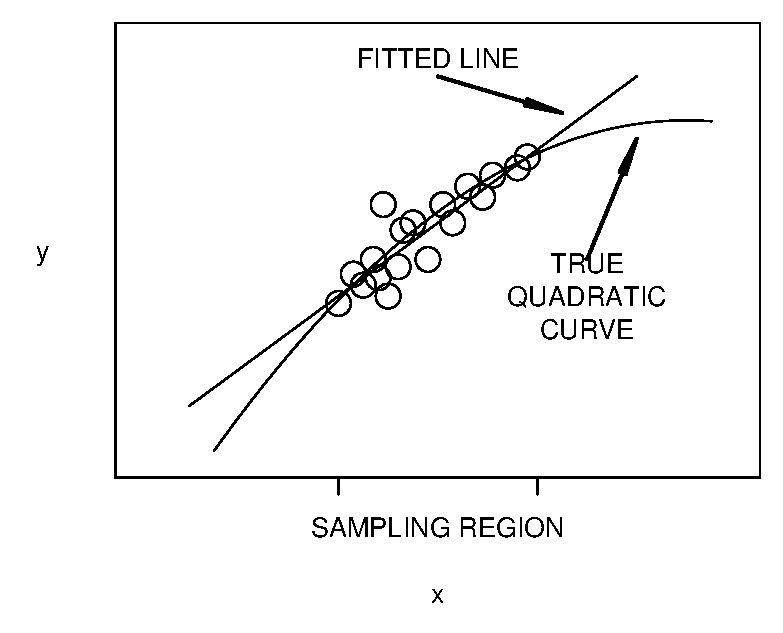
\includegraphics[width=0.6\textwidth]{Chapter6/F6Extrapolation.eps}
    \caption{\label{F6:Extrapolation} \small  Extrapolation outside
of the sampling region may be biased.}
  \end{center}
\end{figure}

Another pitfall due to a limited sampling region, although not a
bias, that can arise is the difficulty in estimating a regression
coefficient. In Chapter 5, we saw that a smaller spread of a
variable, other things equal, means a less reliable estimate of the
slope coefficient associated with that variable. That is, from
Section 5.5.2 or equation \ref{E6:StdErrorBeta}, we see that the
smaller is the spread of $x_{j}$, as measured by $s_{x_{j}}$, the
larger is the standard error of $b_{j},se(b_{j})$. Taken to the
extreme, where $s_{x_{j}}=0$, we might have a situation such as
illustrated in Figure \ref{F6:NoVariation}. For the extreme
situation illustrated in Figure \ref{F6:NoVariation}, there is not
enough variation in $x$ to estimate the corresponding slope
parameter.


\begin{figure}[htp]
  \begin{center}
    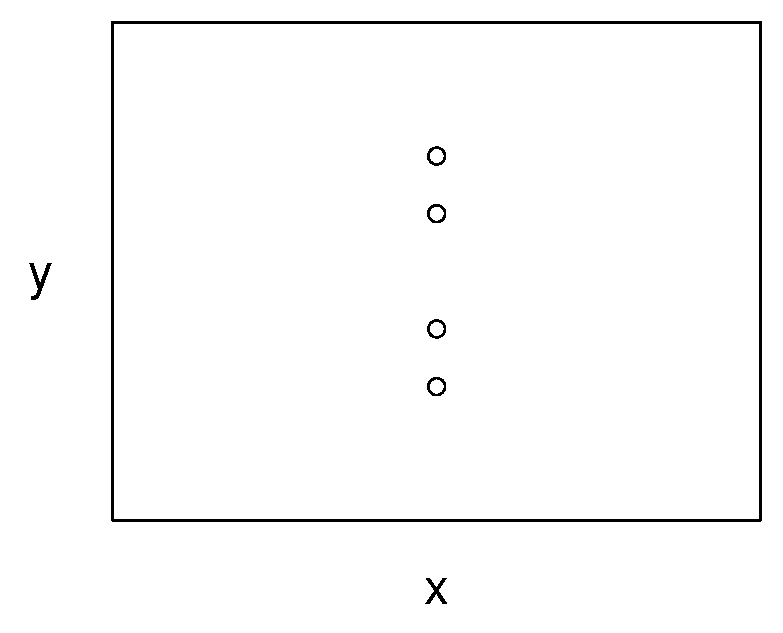
\includegraphics[width=0.4\textwidth]{Chapter6/F6NoVariation.eps}
    \caption{\label{F6:NoVariation} \small  The lack of variation
in $x$ means that we cannot fit a unique line relating $x$ and $y$.}
  \end{center}
\end{figure}




\subsection{Limited Dependent Variables, Censoring and
Truncation}\index{censoring}\index{truncated}

In some applications, the dependent variable is constrained to fall
within certain regions. To see why this is a problem, first recall
that under the linear regression model, the dependent variable
equals the regression function plus a random error. Typically, the
random error is assumed to be approximately normally distributed, so
that the response varies continuously. However, if the outcomes of
the dependent variable are restricted, or limited, then the outcomes
are not purely continuous. This means that our assumption of normal
errors is not strictly correct, and may not even be a good
approximation.

To illustrate, Figure \ref{F6:TwoPartZero} shows a plot of
individual's income ($x$) versus amount of insurance purchased
($y$). The sample in this plot represents two subsamples, those who
purchased insurance, corresponding to $y>0$, and those who did not,
corresponding to ``price'' $y=0$. Fitting a single line to these
data would misinform users about the effects of $x$ on $y$.


\begin{figure}[htp]
    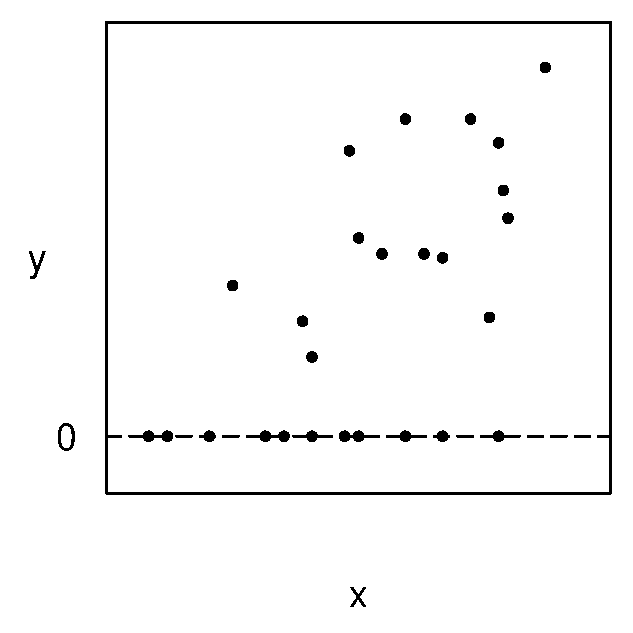
\includegraphics[width=0.45\textwidth]{Chapter6/F6TwoPartZero.eps}   \hfill
    $~~~$
    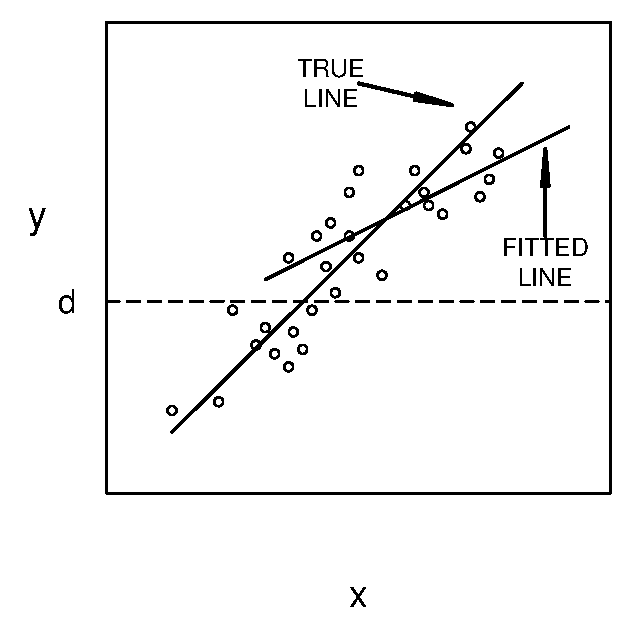
\includegraphics[width=0.45\textwidth]{Chapter6/F6TruncateRegr.eps}
      \parbox[t]{2.5in}{\caption{\label{F6:TwoPartZero}
      \small  When individuals do not purchase anything, they are recorded as $y=0$ sales.}}
\hfill
        \parbox[t]{2.5in}{\caption{\label{F6:TruncateRegr} \small  If the responses below
the horizontal line at $y=d$ are omitted, then the fitted regression
line can be very different from the true regression line.}}
\end{figure}


If we dealt with only those who purchased insurance then we still
would have an implicit lower bound of zero (if an insurance price
must exceed zero). However, prices need be close to this bound for a
given sampling region and thus not represent an important practical
problem. By including several individuals who did not purchase
insurance (and thus spent \$0 on insurance), our sampling region now
clearly includes this lower bound.

There are several ways in which dependent variables can be
restricted, or \textit{censored}. Figure \ref{F6:TwoPartZero}
illustrates the case in which the value of $y$ may be no lower than
zero. As another example, insurance claims are often restricted to
be less than or equal to an upper limit specified in the insurance
policy. If censoring is severe, ordinary least squares produces
biased results. Specialized approaches, known as \textit{censored
regression} models, are described in Chapter 15 to handle this
problem.

Figure \ref{F6:TruncateRegr} illustrates another commonly
encountered limitation on the value of the dependent variable. For
this illustration, suppose that $y$ represents an insured loss and
that $d$ represents the deductible on an insurance policy. In this
scenario, it is common practice for insurers to not record losses
below $d$ (they are typically not reported by policyholders). In
this case, the data are said to be \textit{truncated}. Not
surprisingly, \textit{truncated regression models} are available to
handle this situation. As a rule of thumb, truncated data represent
a more serious source of bias than censored data. When data are
truncated, we do not have values of dependent variables and thus
have less information than when the data are censored. See Chapter
15 for further discussion.


\subsection{Omitted and Endogenous Variables}\index{explanatory
variable!omitted}\index{explanatory variable!endogenous}

Of course, analysts prefer to include all important variables.
However, a common problem is that we may not have the resources nor
the foresight to gather and analyze all the relevant data. Further,
sometimes we are prohibited from including variables. For example,
in insurance rating we are typically precluded from using ethnicity
as a rating variable. Further, there are many mortality and other
decrement tables that are ``uni-sex,'' that is, blind to gender.

Omitting important variables can affect our ability to fit the
regression function; this can affect in-sample (explanation) as well
as out-of-sample (prediction) performance. If the omitted variable
is uncorrelated with other explanatory variables, then the omission
will not affect estimation of regression coefficients. Typically
this is not the case. The Section 3.4.3 Refrigerator Example
illustrates a serious case where the direction of a statistically
significant result was reversed based on the presence of an
explanatory variable. In this example, we found that a cross-section
of refrigerators displayed a significantly positive correlation
between price and the annual energy cost of operating the
refrigerator. This positive correlation was counter-intuitive
because we would hope that higher prices would mean lower annual
expenditures in operating a refrigerator. However, when we included
several additional variables, in particular, measures of the size of
a refrigerator, we found a significantly negative relationship
between price and energy costs. Again, by omitting these additional
variables, there was an important bias when using regression to
understand the relationship between price and energy costs.

Omitted variables can lead to the presence of endogenous explanatory
variables. An exogenous variable is one that can be taken as
``given'' for the purposes at hand.  An endogenous variable is one
that fails the exogeneity requirement. An omitted variable can
affect both the $y$ and the $x$ and in this sense induce a
relationship between the two variables. If the relationship between
$x$ and $y$ is due to an omitted variable, it is difficult to
condition on the $x$ when estimating a model for $y$.

Up to now, the explanatory variables have been treated as
non-stochastic. For many social science applications, it is more
intuitive to consider the $x$'s to be stochastic, and perform
inference conditional on their realizations. For example, under
common sampling schemes, we can estimate the conditional regression
function
\begin{equation*}
\mathrm{E~}\left(y|x_1, \ldots, x_k \right) = \beta_0 + \beta_1 x_1
+ \ldots + \beta_k x_k .
\end{equation*}
This is known as a ``sampling-based'' model.

In the economics literature, Goldberger (1972) defines a
\emph{structural model} as a stochastic model representing a causal
relationship, not a relationship that simply captures statistical
associations. Structural models can readily contain endogenous
explanatory variables. To illustrate, we consider an example
relating claims and premiums. For many lines of business, premium
classes are simply nonlinear functions of exogenous factors such as
age, gender and so forth. For other lines of business, premiums
charged are a function of prior claims history. Consider model
equations that relate one's claims  ($y_{it}, t=1, 2$) to premiums
($x_{it}, t=1, 2$):
 \begin{eqnarray*}
 y_{i2} = \beta_{0,C} + \beta_{1,C} y_{i1} + \beta_{2,C} x_{i2} +
\varepsilon_{i1} \\
 x_{i2} = \beta_{0,P} + \beta_{1,P}  y_{i1} + \beta_{2,P}  x_{i1}
+\varepsilon_{i2} .
 \end{eqnarray*}
In this model, current period ($t=2$) claims and premiums are
affected by the prior period's claims and premiums. This is an
example of a \emph{structural equations} model that requires special
estimation techniques. Our usual estimation procedures are biased!

\linejed\index{examples!race, redlining and automobile insurance
prices}

\textbf{Example: Race, Redlining and Automobile Insurance Prices -
Continued.} Although Harrington and Niehaus (1998) did not find
racial discrimination in insurance pricing, their results on access
to insurance were inconclusive. Insurers offer ``standard'' and
``preferred'' risk contracts to applicants that meet restrictive
underwriting standards, as compared to ``substandard'' risk
contracts where underwriting standards are more relaxed. Expected
claims are lower for standard and preferred risk contracts, and so
premiums are lower, than substandard contracts. Harrington and
Niehaus examined the proportion of applicants offered substandard
contracts, NSSHARE, and found it significantly positively related to
PCTBLACK, the proportion of population black. This suggests evidence
of racial discrimination; they state this to be an inappropriate
interpretation due to omitted variable bias.

Harrington and Niehaus argue that the proportion of applicants
offered substandard contracts should be positively related to
expected claim costs. Further, expected claim costs are strongly
related to PCTBLACK, because minorities in the sample tended to be
lower income. Thus, unobserved variables such as income tend to
drive the positive relationship between NSSHARE and PCTBLACK.
Because the data are analyzed at the zip code level and not at the
individual level, the potential omitted variable bias rendered the
analysis inconclusive.



\linejed

\subsection{Missing Data}\index{sampling!missing data}

In the data examples, illustrations, case studies and exercises of
this text, there are many instances where certain data are
unavailable for analysis, or \textit{missing}. In every instance,
the data were not carelessly lost but were unavailable due to
substantive reasons associated with the data collection. For
example, when we examined stock returns from a cross-section of
companies, we saw that some companies did not have an average five
year earnings per share figure. The reason was simply that they had
not been in existence for five years. As another example, when
examining life expectancies, some countries did not report the total
fertility rate because they lacked administrative resources to
capture this data. Missing data are an inescapable aspect of
analyzing data in the social sciences.

When the reason for the lack of availability of data is unrelated to
actual data values, the data are said to be \textit{missing at
random}. There are a variety of techniques for handling missing at
random data, none of which are clearly superior to the others. One
``technique'' is to simply ignore the problem. Hence, missing at
random is sometimes called the \textit{ignorable case} of missing
data.\index{sampling!missing at random}\index{sampling!ignorable
case}

If there are only a few missing data, compared to the total number
available, a widely employed strategy is to delete the observations
corresponding to the missing data. Assuming that the data are
missing at random, little information is lost by deleting a small
portion of the data. Further, with this strategy, we need not make
additional assumptions about the relationships among the data.

If the missing data are primarily from one variable, we can consider
omitting this variable. Here, the motivation is that we lose less
information when omitting this variable as compared to retaining the
variable but losing the observations associated with the missing
data.\index{sampling!impute}

Another strategy is to fill in, or \textit{impute}, missing data.
There are many variations of the imputation strategy. All assume
some type of relationships among the variables in addition to the
regression model assumptions. Although these methods yield
reasonable results, note that any type of filled-in values do not
yield the same inherent variability as the real data. Thus, results
of analyses based on imputed values often reflect less variability
than those with real data.

\linejed\index{datasets!insurance company expenses}

\textbf{Example: Insurance Company Expenses - Continued.} When
examining company financial information, analysts commonly are
forced to omit substantial amounts of information when using
regression models to search for relationships. To illustrate, Segal
(2002) examined life insurance financial statements from data
provided by the National Association of Insurance Commissioners
(NAIC). He initially considered 733 firm-year observations over the
period 1995-1998. However, 154 observations were excluded because of
inconsistent or negative premiums, benefits and other important
explanatory variables. Small companies representing 131 observations
were also excluded. Small companies consist of fewer than 10
employees and agents, operating costs less than \$1 million or fewer
than 1,000 life policies sold. The resulting sample was $n=448$
observations. The sample restrictions were based on explanatory
variables - this procedure does not necessarily bias results. Segal
argued that his final sample remained representative of the
population of interest. There were about 110 firms in each of
1995-1998. In 1998, aggregate assets of the firms in the sample
represent approximately \$650 billion, a third of the life insurance
industry.

\linejed


\section{Missing Data Models}

To understand the mechanisms that lead to unplanned nonresponse, we
model it stochastically. Let $r_i$ be a binary variable for the
$i$th observation, with a one indicating that this response is
observed and a zero indicating that the response is missing. Let
$\mathbf{r} = (r_1, \ldots, r_n)^{\prime}$  summarize the data
availability for all subjects. The interest is in whether or not the
responses influence the missing data mechanism. For notation, we use
$\mathbf{Y} = (y_1, \ldots, y_n)^{\prime}$  to be the collection of
all potentially observed responses.

\subsection{Missing at Random}\index{sampling!missing completely at random, MCAR}

In the case where $\mathbf{Y}$ does not affect the distribution of
$\mathbf{r}$, we follow Rubin (1976) and call this case
\emph{missing completely at random (MCAR)}. Specifically, the
missing data are MCAR if $\mathrm{f}(\mathbf{r} | \mathbf{Y}) =
\mathrm{f}(\mathbf{r})$, where f(.) is a generic probability mass
function. An extension of this idea is in Little (1995), where the
adjective ``covariate dependent'' is added when $\mathbf{Y}$ does
not affect the distribution of $\mathbf{r}$, conditional on the
covariates. If the covariates are summarized as $\mathbf{X}$, then
the condition corresponds to the relation $\mathrm{f}(\mathbf{r} |
\mathbf{Y, X}) = \mathrm{f}(\mathbf{r | X})$. To illustrate this
point, consider an example of Little and Rubin (1987) where
$\mathbf{X}$ corresponds to age and $\mathbf{Y}$ corresponds to
income of all potential observations. If the probability of being
missing does not depend on income, then the missing data are MCAR.
If the probability of being missing varies by age but does not by
income over observations within an age group, then the missing data
are covariate dependent MCAR. Under the latter specification, it is
possible for the missing data to vary by income. For example,
younger people may be less likely to respond to a survey. This shows
that the ``missing at random'' feature depends on the purpose of the
analysis. Specifically, it is possible that an analysis of the joint
effects of age and income may encounter serious patterns of missing
data whereas an analysis of income controlled for age suffers no
serious bias patterns.

Little and Rubin (1987) advocate modeling the missing data
mechanisms. To illustrate, consider a likelihood approach using a
selection model for the missing data mechanism. Now, partition
$\mathbf{Y}$ into observed and missing components using the notation
$\mathbf{Y} =\{\mathbf{Y}_{obs}, \mathbf{Y}_{miss}\}$. With the
likelihood approach, we base inference on the observed random
variables. Thus, we use a likelihood proportional to the joint
function $\mathrm{f}(\mathbf{r}, \mathbf{Y}_{obs})$. We also specify
a \emph{selection model} by specifying the conditional mass function
$\mathrm{f}(\mathbf{r} | \mathbf{Y})$.

Suppose that the observed responses and the selection model
distributions are characterized by a vectors of parameters
$\boldsymbol \theta$ and $\boldsymbol \psi$ , respectively. Then,
with the relation $\mathrm{f}(\mathbf{r}, \mathbf{Y}_{obs},
\boldsymbol \theta, \boldsymbol \psi)$ $ =
\mathrm{f}(\mathbf{Y}_{obs}, \boldsymbol \theta) \times
\mathrm{f}(\mathbf{r} | \mathbf{Y}_{obs}, \boldsymbol \psi)$, we may
express the log likelihood of the observed random variables as

\begin{equation*}
L(\boldsymbol \theta, \boldsymbol \psi) = \mathrm{ln~}
\mathrm{f}(\mathbf{r}, \mathbf{Y}_{obs}, \boldsymbol \theta,
\boldsymbol \psi) = \mathrm{ln~} \mathrm{f}(\mathbf{Y}_{obs},
\boldsymbol \theta) + \mathrm{ln~} \mathrm{f}(\mathbf{r} |
\mathbf{Y}_{obs}, \boldsymbol \psi).
\end{equation*}
(See Section 11.9 if you would like a refresher on likelihood
inference.) In the case where the data are MCAR, then
$\mathrm{f}(\mathbf{r} | \mathbf{Y}_{obs}, \boldsymbol \psi) =
\mathrm{f}(\mathbf{r} | \boldsymbol \psi)$ does not depend on
$\mathbf{Y}_{obs}$. Little and Rubin (1987) also consider the case
where the selection mechanism model distribution does not depend on
$\mathbf{Y}_{miss}$ but may depend on $\mathbf{Y}_{obs}$. In this
case, they call the \emph{data missing at random
(MAR)}.\index{sampling!missing at random, MAR}

In both the MAR and MCAR cases, we see that the likelihood may be
maximized over the parameters, separately for each case. In
particular, if one is only interested in the maximum likelihood
estimator of $\boldsymbol \theta$, then the selection model
mechanism may be ``ignored.'' Hence, both situations are often
referred to as the \emph{ignorable case}.\index{sampling!ignorable
case}

\linejed\index{examples!dental expenditures}

\textbf{Example: Dental Expenditures.}\ecaptionjed{Dental
Expenditures} Let $y$ represent a household's annual dental
expenditure and $x$ represent income. Consider the following five
selection mechanisms.
\begin{itemize}
  \item The household is not selected (missing) with probability without
regard to the level of dental expenditure. In this case, the
selection mechanism is MCAR.
  \item The household is not selected if the dental expenditure is less
than \$100. In this case, the selection mechanism depends on the
observed and missing response. The selection mechanism cannot be
ignored.
  \item The household is not selected if the income is less
than \$20,000. In this case, the selection mechanism is MCAR,
covariate dependent. That is, assuming that the purpose of the
analysis is to understand dental expenditures conditional on
knowledge of income, stratifying based on income does not seriously
bias the analysis.
  \item The probability of a household being selected increases
with dental expenditure. For example, suppose the probability of
being selected is a linear function of $\exp(\psi  y_i)/(1+ \exp
(\psi y_i))$. In this case, the selection mechanism depends on the
observed and missing response. The selection mechanism cannot be
ignored.
  \item The household is followed over $T$ = 2
periods. In the second period, a household is not selected if the
first period expenditure is less than \$100. In this case, the
selection mechanism is MAR. That is, the selection mechanism is
based on an observed response.
\end{itemize}

\linejed

\bigskip

The second and fourth selection mechanisms represent situations
where the selection mechanism must be explicitly modeled; these are
non-ignorable cases. In these situations without explicit
adjustments, procedures that ignore the selection effect may produce
seriously biased results. To illustrate a correction for selection
bias in a simple case, we outline an example due to Little and Rubin
(1987). Section \ref{S6:NonIgnore} describes additional mechanisms.

\linejed\index{examples!historical heights}

\textbf{Example: Historical Heights.}\ecaptionjed{Historical
Heights} Little and Rubin (1987) discuss data due to Wachter and
Trusell (1982) on $y$, the height of men recruited to serve in the
military. The sample is subject to censoring in that minimum height
standards were imposed for admission to the military. Thus, the
selection mechanism is
\begin{equation*}
r_i = \left\{
              \begin{array}{ll}
                1 & y_i > c_i \\
                0 & \mathrm{otherwise} \\
              \end{array}
            \right. ,
\end{equation*}
where $c_i$ is the known minimum height standard imposed at the time
of recruitment. The selection mechanism is non-ignorable because it
depends on the individual's height, $y$.

For this example, additional information is available to provide
reliable model inference. Specifically, based on other studies of
male heights, we may assume that the population of heights is
normally distributed. Thus, the likelihood of the observables can be
written down and inference may proceed directly. To illustrate,
suppose that $c_i = c$ is constant. Let $\mu$ and $\sigma$ denote
the mean and standard deviation of $y$. Further suppose that we have
a random sample of $n + m$ men in which $m$ men fall below the
minimum standard height $c$ and we observe $\mathbf{Y}_{obs} = (y_1,
\ldots, y_n)^{\prime} $. The joint distribution for observables is

\begin{eqnarray*}
\mathrm{f}(\mathbf{r}, \mathbf{Y}_{obs}, \mu, \sigma) &=&
\mathrm{f}(\mathbf{Y}_{obs}, \mu, \sigma) \times
\mathrm{f}(\mathbf{r} | \mathbf{Y}_{obs}) \\
&=& \left\{ \prod_{i=1}^n   \mathrm{f}(y_i | y_i > c) \times
\mathrm{Pr}(y_i > c) \right\}
 \times \left\{\mathrm{Pr}(y_i \leq c)\right\}^m.
\end{eqnarray*}
Now, let $\phi$ and $\Phi$ represent the density and distribution
function for the standard normal distribution. Thus, the
log-likelihood is
\begin{eqnarray*}
L(\mu, \sigma) &=& \mathrm{ln~} \mathrm{f}(\mathbf{r},
\mathbf{Y}_{obs}, \mu, \sigma) \\
&=& \sum_{i=1}^n \mathrm{ln}\left\{ \frac{1}{\sigma} \phi \left(
\frac{y_i-\mu}{\sigma} \right)
 \right\}
 +  m~ \mathrm{ln}\left\{ \Phi \left(
\frac{c-\mu}{\sigma}\right) \right\}
\end{eqnarray*}
This is easy to maximize in $\mu$ and $\sigma$. If one ignored the
censoring mechanisms, then one would derive estimates of the
observed data from the ``log likelihood,''
\begin{equation*}
\sum_{i=1}^n \mathrm{ln}\left\{ \frac{1}{\sigma} \phi \left(
\frac{y_i-\mu}{\sigma} \right)
 \right\},
\end{equation*}
yielding different, and biased, results.

\linejed

\subsection{Non-Ignorable Missing Data}\label{S6:NonIgnore}\index{sampling!non-ignorable
case}

For non-ignorable missing data, Little (1995) recommends:
    \begin{itemize}
      \item Avoid missing responses whenever possible by using appropriate
follow-up procedures.
      \item Collect covariates that are useful for predicting missing
values.
      \item Collect as much information as possible regarding the
nature of the missing data mechanism.
    \end{itemize}
For the third point, if little is known about the missing data
mechanism, then it is difficult to employ a robust statistical
procedure to correct for the selection bias.

There are many models of missing data mechanisms. A general overview
appears in Little and Rubin (1987). Little (1995) surveys the
problem of attrition. Rather than survey this developing literature,
we give a widely used model of non-ignorable missing data.

\subsubsection*{Heckman Two-Stage Procedure}\index{sampling!Heckman procedure}

Heckman (1976) assumes that the sampling response mechanism is
governed by the latent (unobserved) variable $r_i^{\ast}$ where
\begin{equation*}
r_i^{\ast} = \mathbf{z}_i^{\prime} \boldsymbol \gamma + \eta _i.
\end{equation*}
The variables in $\mathbf{z}_i$ may or may not include the variables
in $\mathbf{x}_i$. We observe $y_i$ if $r_i^{\ast}>0$, that is, if
$r_i^{\ast}$ crosses the threshold 0. Thus, we observe
\begin{equation*}
r_i = \left\{
              \begin{array}{ll}
                1 & r_i^{\ast}>0 \\
                0 & \mathrm{otherwise} \\
              \end{array}
            \right. .
\end{equation*}
To complete the specification, we assume that
{($\varepsilon_i,\eta_i$)} are identically and independently
distributed, and that the joint distribution of
($\varepsilon_i,\eta_i$)  is bivariate normal with means zero,
variances $\sigma^2$ and $\sigma_{\eta}^2$ and correlation $\rho$.
Note that if the correlation parameter $\rho$ equals zero, then the
response and selection models are independent. In this case, the
data are MCAR and the usual estimation procedures are unbiased and
asymptotically efficient.

Under these assumptions, basic multivariate normal calculations show
that
\begin{equation*}
\mathrm{E~}(y_i | r_i^{\ast}>0) = \mathbf{x}_i^{\prime} \boldsymbol
\beta + \beta_{\lambda} \lambda(\mathbf{z}_i^{\prime} \boldsymbol
\gamma),
\end{equation*}
where $\beta_{\lambda} = \rho \sigma$ and
$\lambda(a)=\phi(a)/\Phi(a)$. Here, $\lambda(.)$ is the inverse of
the so-called ``Mills ratio.'' This calculation suggests the
following two-step procedure for estimating the parameters of
interest.

\bigskip

\boxedjed

\textit{Heckman's Two-Stage Procedure}
\begin{enumerate}
  \item Use the data {($r_i, \mathbf{z}_i$)} and a probit regression model to estimate $\boldsymbol \gamma$. Call this
estimator $\mathbf{g}_H$.
  \item Use the estimator from stage (i) to create a new
explanatory variable, $x_{i,K+1} =
\lambda(\mathbf{z}_i^{\prime}\mathbf{g}_H)$. Run a regression model
using the $K$ explanatory variables $\mathbf{x}_i$ as well as the
additional explanatory variable $x_{i,K+1}$. Use $\mathbf{b}_H$ and
$b_{\lambda,H}$ to denote the estimators of $ \boldsymbol \beta$ and
$\beta_{\lambda}$, respectively.
\end{enumerate}
\end{boxedminipage}

\bigskip

\noindent Chapter 11 will introduce probit regressions. We also note
that the two-step method does not work in absence of covariates to
predict the response and, for practical purposes, requires variables
in $\mathbf{z}$ that are not in $\mathbf{x}$ (see Little and Rubin,
1987).

To test for selection bias, we may test the null hypothesis
$H_0:\beta_{\lambda}=0$ in the second stage due to the relation
$\beta_{\lambda}= \rho \sigma$. When conducting this test, one
should use heteroscedasticity-corrected standard errors. This is
because the conditional variance $\mathrm{Var}(y_i | r_i^{\ast}>0)$
depends on the observation $i$. Specifically, $\mathrm{Var}(y_i |
r_i^{\ast}>0) = \sigma^2 (1-\rho^2 \delta_i),$ where $\delta_i=
\lambda_i(\lambda_i + \mathbf{z}_i^{\prime} \boldsymbol \gamma)$ and
$\lambda_i = \phi(\mathbf{z}_i^{\prime} \boldsymbol
\gamma)/\Phi(\mathbf{z}_i^{\prime} \boldsymbol
\gamma).$\index{heteroscedasticity}


This procedure assumes normality for the selection latent variables
to form the augmented variables. Other distribution forms are
available in the literature, including the logistic and uniform
distributions. A deeper criticism, raised by Little (1985), is that
the procedure relies heavily on assumptions that cannot be tested
using the data available. This criticism is analogous to the
historical heights example where we relied heavily on the normal
curve to infer the distribution of heights below the censoring
point. Despite these criticisms, Heckman's procedure is widely used
in the social sciences.

\subsubsection*{EM algorithm}

Section \ref{S6:NonIgnore} has focused on introducing specific
models of non-ignorable nonresponse. General robust models of
nonresponse are not available. Rather, a more appropriate strategy
is to focus on a specific situation, collect as much information as
possible regarding the nature of the selection problem and then
develop a model for this specific selection problem.

The EM algorithm is a computational device for computing model
parameters. Although specific to each model, it has found
applications in a wide variety of models involving missing data.
Computationally, the algorithm iterates between the ``E,'' for
conditional expectation, and ``M,'' for maximization, steps. The E
step finds the conditional expectation of the missing data given the
observed data and current values of the estimated parameters. This
is analogous to the time-honored tradition of imputing missing data.
A key innovation of the EM algorithm is that one imputes sufficient
statistics for missing values, not the individual data points. For
the M step, one updates parameter estimates by maximizing an
observed log likelihood. Both the sufficient statistics and the log
likelihood depend on the model specification.

Many introductions of the EM algorithm are available in the
literature. Little and Rubin (1987) provide a detailed treatment.


\section{Application: Risk Managers' Cost Effectiveness}\ecaptionjed{Risk Managers' Cost Effectiveness}

This section examines data from a survey on the cost effectiveness
of risk management practices. Risk management practices are
activities undertaken by a firm to minimize the potential cost of
future losses, such as the event of a fire in a warehouse or an
accident that injures employees. This section develops a model that
can be used to make statements about cost of managing risks.

An outline of the regression modeling process is as follows. We
begin by providing an introduction to the problem and giving some
brief background on the data. Certain prior theories will lead us to
present a preliminary model fit. Using diagnostic techniques, it
will be evident that several assumptions underpinning this model are
not in accord with the data. This will lead us to go back to the
beginning and start the analysis from scratch. Things that we learn
from a detailed examination of the data will lead us to postulate
some revised models. Finally, to communicate certain aspects of the
new model, we will explore graphical presentations of the
recommended model.

\subsubsection*{Introduction}

\empexjed{RiskSurvey}\index{datasets!risk managers cost
effectiveness}

The data for this study were provided by Professor Joan Schmit and
are discussed in more detail in the paper, ``Cost effectiveness of
risk management practices,'' Schmit and Roth (1990). The data are
from a questionnaire that was sent to 374 risk managers of large
U.S.-based organizations. The purpose of the study was to relate
cost effectiveness to management's philosophy of controlling the
company's exposure to various property and casualty losses, after
adjusting for company effects such as size and industry type.

First, some caveats. Survey data are often based on samples of
convenience, not probability samples. Just as with all observational
data sets, regression methodology is a useful tool for summarizing
data. However, we must be careful when making inferences based on
this type of data set. For this particular survey, 162 managers
returned completed surveys resulting in a good response rate of
$43\%$. However, for the variables included in the analysis (defined
below), only 73 forms were completed resulting in a complete
response rate of $20\%$. Why such a dramatic difference? Managers,
like most people, typically do not mind responding to queries about
their attitudes, or opinions, about various issues. When questioned
about hard facts, in this case company asset size or insurance
premiums, either they considered the information proprietary and
were reluctant to respond even when guaranteed anonymity or they
simply were not willing to take the time to look up the information.
From a surveyor's standpoint, this is unfortunate because typically
``attitudinal'' data are fuzzy (high variance compared to the mean)
as compared to hard financial data. The tradeoff is that the latter
data are often hard to obtain. In fact, for this survey, several
pre-questionnaires were sent to ascertain managers' willingness to
answer specific questions. From the pre-questionnaires, the
researchers severely reduced the number of financial questions that
they intended to ask.

A measure of risk management cost effectiveness, FIRMCOST, is the
dependent variable. This variable is defined as total property and
casualty premiums and uninsured losses as a percentage of total
assets. It is a proxy for annual expenditures associated with
insurable events, standardized by company size. Here, for the
financial variables, ASSUME is the per occurrence retention amount
as a percentage of total assets, CAP indicates whether the company
owns a captive insurance company, SIZELOG is the logarithm of total
assets and INDCOST is a measure of the firm's industry risk.
Attitudinal variables include CENTRAL, a measure of the importance
of the local managers in choosing the amount of risk to be retained
and SOPH, a measure of the degree of importance in using analytical
tools, such as regression, in making risk management decisions.

In the paper, the researchers described several weaknesses of the
definitions used but argue that these definitions provide useful
information, based on the willingness of risk managers to obtain
reliable information. The researchers also described several
theories concerning relationships that may be confirmed by the data.
Specifically, they hypothesized:
\begin{itemize}

\item There exists an inverse relationship between the risk
retention (ASSUME) and cost (FIRMCOST). The idea behind this theory
is that larger retention amounts should mean lower expenses to a
firm, resulting in lower costs.

\item  The use of a captive insurance company (CAP) results in lower costs.
Presumably, a captive is used only when cost effective and
consequently, this variable should indicate lower costs if used
effectively.

\item  There exists an inverse relationship between the measure of
centralization (CENTRAL) and cost (FIRMCOST). Presumably, local
managers would be able to make more cost effective decisions because
they are more familiar with local circumstances regarding risk
management than centrally located managers.

\item  There exists an inverse relationship between the measure of
sophistication (SOPH) and cost (FIRMCOST). Presumably, more
sophisticated analytical tools help firms to manage risk better,
resulting in lower costs.
\end{itemize}

\subsubsection*{Preliminary Analysis}

To test the theories described above, the regression analysis framework can
be used. To do this, posit the model

\begin{center}
\begin{eqnarray*}
\text{FIRMCOST} &=&\beta_0 +\beta_1 \text{ ASSUME}+\beta _{2}\text{ CAP}%
+\beta _{3}\text{ SIZELOG}+\beta_4\text{ INDCOST} \\
&&+\beta_5\text{ CENTRAL}+\beta_6\text{ SOPH}+ \varepsilon.
\end{eqnarray*}
\end{center}

With this model, each theory can be interpreted in terms of
regression coefficients. For example, $\beta_1 $ can be interpreted
as the expected change in cost per unit change in retention level
(ASSUME). Thus, if the first hypothesis is true, we expect $\beta_1
$ to be negative. To test this, we can estimate $b_{1}$ and use our
tests of hypotheses machinery to decide if $b_{1}$ is significantly
less than zero. The variables SIZELOG and INDCOST are included in
the model to control for the effects of these variables. These
variables are not directly under a risk manager's control and thus
are not of primary interest. However, inclusion of these variables
can account for an important part of the variability.

Data from 73 managers was fit using this regression model. Table
\ref{T6:FirmRiskPrelim} summarizes the fitted model.

\begin{table}[h]
\scalefont{0.9} \caption{\label{T6:FirmRiskPrelim} Regression
Results from a Preliminary Model Fit}
\begin{tabular}{l|rrr}
\hline
 &  & Standard &  \\
Variable & Coefficient & Error & $t$-statistic \\
\hline
INTERCEPT & 59.76 & 19.1 & 3.13 \\
ASSUME & -0.300 & 0.222 & -1.35 \\
CAP & 5.50 & 3.85 & 1.43 \\
SIZELOG & -6.84 & 1.92 & -3.56 \\
INDCOST & 23.08 & 8.30 & 2.78 \\
CENTRAL & 0.133 & 1.44 & 0.89 \\
SOPH & -0.137 & 0.347 & -0.39 \\
\hline
\end{tabular}
\scalefont{1.1111}  \end{table}


\noindent The adjusted coefficient of determination is $R_{a}^{2}=18.8\%$, the \textit{%
F-}ratio is 3.78 and the residual standard deviation is $s=14.56$.

Based on the summary statistics from the regression model, we can
conclude that the measures of centralization and sophistication do
not have an impact on our measure of cost effectiveness. For both of
these variables the \textit{t-}ratio is low, less than 1.0 in
absolute value. The effect of risk retention seems only somewhat
important. The coefficient has the appropriate sign although is only
1.35 standard errors below zero. This would not be considered
statistically significant at the 5\% level, although it would be at
the 10\% level (the \textit{p-}value is 9\%). Perhaps most
perplexing is the coefficient associated with the CAP variable. We
theorized that this coefficient would be negative. However, in our
analysis of the data, the coefficient turns out to be positive and
is 1.43 standard errors above zero. This not only leads us to
disaffirm our theory, but also to search for new ideas that are in
accord with the information learned from the data. Schmit and Roth
suggest reasons that may help us interpret the results of our
hypothesis testing procedures. For example, they suggest that
managers in the sample may not have the most sophisticated tools
available to them when managing risks, resulting in an insignificant
coefficient associated with SOPH. They also discussed alternative
suggestions, as well as interpretations for the other results of the
tests of hypotheses.

How robust is this model? Section 6.2 emphasized some of the dangers
of working with an inadequate model. Some readers may feel
uncomfortable with the model selected above because two out of the
six variables have \textit{t-}ratios less than 1 in absolute value
and four out of six have \textit{t-}ratios less than 1.5 in absolute
value. Perhaps even more important, histograms of the standardized
residuals and leverages, in Figure \ref{F6:ResidLeverage1}, show
several observations to be outliers and high leverage points. To
illustrate, the largest residual turns out to be $e_{15}=83.73$. The
error sum of squares is $Error~SS$ = $(n-(k+1))s^{2}$ =
$(73-7)(14.56)^{2}=13,987$. Thus, the
15th observation represents 50.1\% of the error sum of squares $%
(=83.73^{2}/13,987)$, suggesting that this 1 observation out of 73
has a dominant impact on the model fit. Further, plots of
standardized residuals versus fitted values, not presented here,
displayed evidence of heteroscedastic residuals. Based on these
observations, it seems reasonable to assess the robustness of the
model.


\begin{figure}[htp]
  \begin{center}
   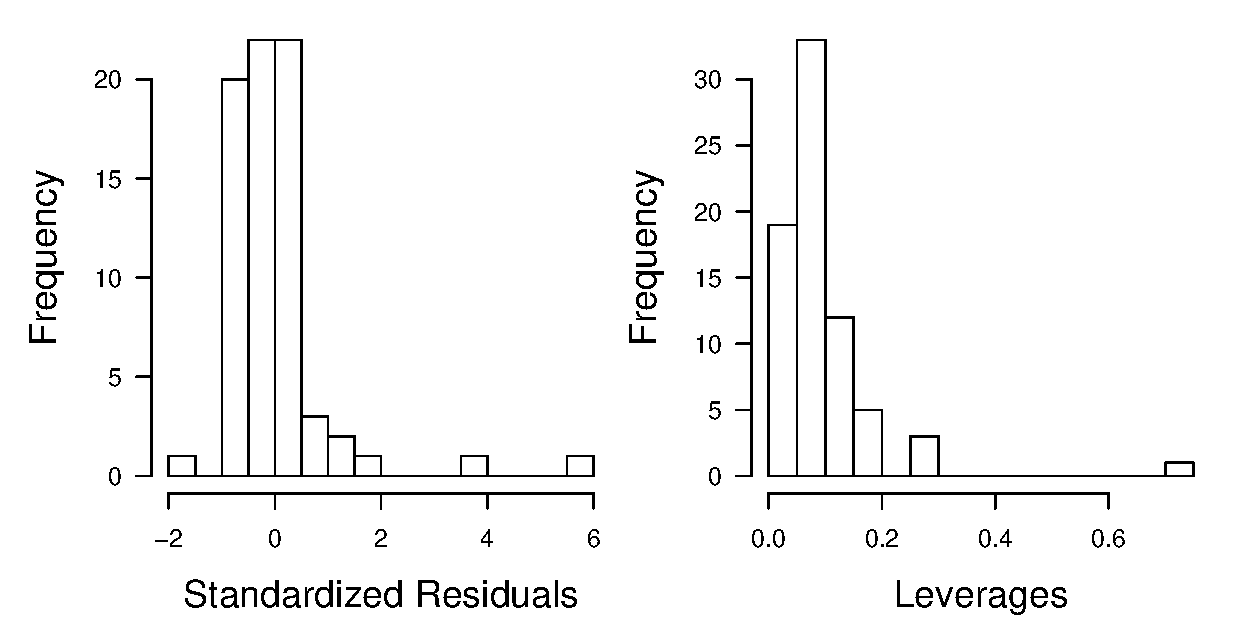
\includegraphics[width=.6\textwidth]{Chapter6/F6ResidLeverage1.eps}
    \caption{\label{F6:ResidLeverage1}
    \small Histograms of standardized residuals and leverages from a preliminary regression model fit.}
  \end{center}
\end{figure}



\subsubsection*{Back to the Basics}

To get a better understanding of the data, we begin by examining the
basic summary statistics in Table \ref{T6:RiskSumStats} and
corresponding histograms in Figure \ref{F6:SurveyBasicPlot}. From
Table \ref{T6:RiskSumStats}, the largest value of FIRMCOST is 97.55,
which is more than five standard deviations above the mean
$[10.97+5(16.16)=91.77]$. An examination of the data shows that this
point is observation \#15, the same observation that was an outlier
in the preliminary regression fit. However, the histogram of
FIRMCOST in Figure \ref{F6:SurveyBasicPlot} reveals that this is not
the only unusual point. Two other observations have unusually large
values of FIRMCOST, resulting in a distribution that is skewed to
the right. The histogram, in Figure \ref{F6:SurveyBasicPlot}, of the
ASSUME variable shows that this distribution is also skewed to the
right, possibly due solely to two large observations. From the basic
summary statistics in Table \ref{T6:RiskSumStats}, we see that the
largest value of ASSUME is more than seven standard deviations above
the mean. This observation may well turn out to be influential in
subsequent regression model fitting. The scatterplot of FIRMCOST
versus ASSUME in Figure \ref{F6:SurveyBasicPlot} tells us that the
observation with the largest value of FIRMCOST is not the same as
the observation with the largest value of ASSUME.



\begin{table}[h]\scalefont{0.9}
\caption{\label{T6:RiskSumStats} Summary Statistics of $n=73$ Risk
Management Surveys}
\begin{tabular}{lrrrrr}
\hline
&  &    & Standard &  &  \\
&  Mean & Median & Deviation & Minimum & Maximum \\ \hline FIRMCOST
&  10.97 & 6.08 & 16.16 &
0.20 & 97.55 \\
ASSUME &   2.574 & 0.510 & 8.445 &
0.000 & 61.820 \\
CAP & 0.342 & 0.000 & 0.478 &
0.000 & 1.000 \\
SIZELOG &   8.332 & 8.270 & 0.963 &
5.270 & 10.600 \\
INDCOST &   0.418 & 0.340 & 0.216 &
0.090 & 1.220 \\
CENTRAL &   2.247 & 2.200 & 1.256 &
1.000 & 5.000 \\
SOPH &  21.192 &23.00 & 5.304 & 5.000 & 31.000 \\ \hline
\end{tabular}

{\small \textit{Source}: Schmit and Roth, (1990)} \scalefont{1.1111}
\end{table}


From the histograms of SIZELOG, INDCOST, CENTRAL, and SOPH, we see
that these distributions are not heavily skewed. Taking logarithms
of the size of total company assets has served to make the
distribution more symmetric than in the original units. From the
histogram and summary statistics, we see that CENTRAL is a discrete
variables, taking on values one through five. The other discrete
variable is CAP, a binary variable taking values only zero and one.
The histogram and scatter plot corresponding to CAP is not presented
here. It is more informative to provide a \textit{table of means} of
each variable by levels of CAP, as in Table \ref{T6:RiskByCap}. From
this table, we see that 25 of the 73 companies surveyed own captive
insurers. Further, on one
hand, the average FIRMCOST for those companies with captive insurers $($CAP $%
=1)$ is larger than those without $($CAP $=0)$. On the other hand,
when moving to the logarithmic scale, the opposite is true; that is,
average COSTLOG for those companies with captive insurers $($CAP
$=1)$ is larger than those without $($CAP $=0)$.

\begin{table}[h]\scalefont{0.8}
\caption{\label{T6:RiskByCap} Table of Means by Level of CAP}
\begin{tabular}{lcrrrrrrr}
\hline
& $n$ &FIRMCOST&ASSUME&SIZELOG&INDCOST&CENTRAL&SOPH&COSTLOG\\
CAP=0 & 48 &  9.954 & 1.175 & 8.197 & 0.399 & 2.250 & 21.521 & 1.820 \\
CAP=1 & 25 & 12.931 & 5.258 & 8.592 & 0.455 & 2.240 & 20.560 & 1.595 \\
TOTAL & 73 & 10.973 & 2.574 & 8.332 & 0.418 & 2.247 & 21.192 & 1.743 \\
\hline
\end{tabular}
\scalefont{1.25}
\end{table}

\begin{figure}[htp]
  \begin{center}
   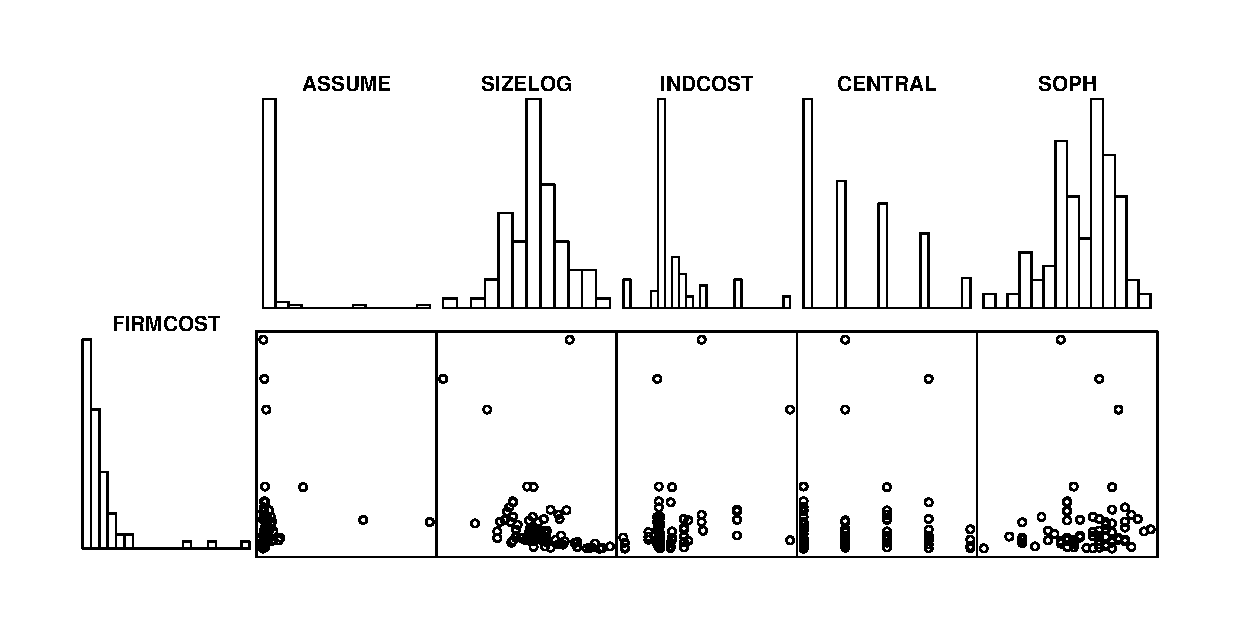
\includegraphics[width=1\textwidth]{Chapter6/F6SurveyBasicPlot.eps}
    \caption{\label{F6:SurveyBasicPlot} \small {Histograms and
    scatter plots of FIRMCOST and several explanatory variables. The
    distributions of FIRMCOST and ASSUME are heavily skewed to the
    right. There is a negative relationship between FIRMCOST and
    SIZELOG, although nonlinear.}}
      \end{center}
\end{figure}


When examining relationships between pairs of variables, in Figure
\ref{F6:SurveyBasicPlot} we see some of the relationships that were
evident from preliminary regression fit. There is an inverse
relationship between FIRMCOST and SIZELOG, and the scatterplot plot
suggests this relationship may be nonlinear. There is also a mild
positive relationship between FIRMCOST and INDCOST and no apparent
relationships between FIRMCOST and any of the other explanatory
variables. These observations are reinforced by the table of
correlations given in Table \ref{T6:RiskCorrStats}. Note that the
table masks a feature that is evident in the scatter plots, the
effect of the unusually large observations.


\begin{table}[h]
\scalefont{0.8} \caption{\label{T6:RiskCorrStats} Correlation
Matrix}
\begin{tabular}{lrrrrrrr}
\hline & COSTLOG & FIRMCOST & ASSUME & CAP & SIZELOG & INDCOST &
CENTRAL \\ \hline FIRMCOST & \multicolumn{1}{r}{0.713} &
 &  &  &  & &  \\
ASSUME & \multicolumn{1}{r}{0.165} & \multicolumn{1}{r}{0.039} &
 &  &  &  &  \\
CAP & \multicolumn{1}{r}{-0.088} & \multicolumn{1}{r}{0.088} &
\multicolumn{1}{r}{0.231} &  &  &  &  \\
SIZELOG & \multicolumn{1}{r}{-0.637} & \multicolumn{1}{r}{-0.366} &
\multicolumn{1}{r}{-0.209} & \multicolumn{1}{r}{0.196} &  &  &  \\
INDCOST & \multicolumn{1}{r}{0.395} & \multicolumn{1}{r}{0.326} &
\multicolumn{1}{r}{0.249} & \multicolumn{1}{r}{0.122} & \multicolumn{1}{r}{
-0.102} &  &  \\
CENTRAL & \multicolumn{1}{r}{-0.054} & \multicolumn{1}{r}{0.014} &
\multicolumn{1}{r}{-0.068} & \multicolumn{1}{r}{-0.004} & \multicolumn{1}{r}{
-0.080} & \multicolumn{1}{r}{-0.085} &  \\
SOPH & \multicolumn{1}{r}{0.144} & \multicolumn{1}{r}{0.048} &
\multicolumn{1}{r}{0.062} & \multicolumn{1}{r}{-0.087} & \multicolumn{1}{r}{
-0.209} & \multicolumn{1}{r}{0.093} & \multicolumn{1}{r}{0.283} \\ \hline
\end{tabular}\scalefont{1.25}
\end{table}


Because of the skewness of the distribution and the effect of the
unusually large observations, a transformation of the response
variable might lead to fruitful results. Figure \ref{F6:HistCostLog}
is the histogram of COSTLOG, defined to be the logarithm of
FIRMCOST. The distribution is much less skewed than the distribution
of FIRMCOST. The variable COSTLOG was also included in the
correlation matrix in Table \ref{T6:RiskCorrStats}. From this table,
the relationship between SIZELOG appears to be stronger with COSTLOG
than with FIRMCOST. Figure \ref{F6:CostLogPlots} shows several
scatter plots illustrating the relationship between COSTLOG and the
explanatory variables. The relationship between COSTLOG and SIZELOG
appears to be linear. It is easier to interpret these scatter plots
than those in Figure \ref{F6:SurveyBasicPlot} due to the absence of
the large unusual values of the dependent variable.

\begin{figure}[htp]
  \begin{center}
   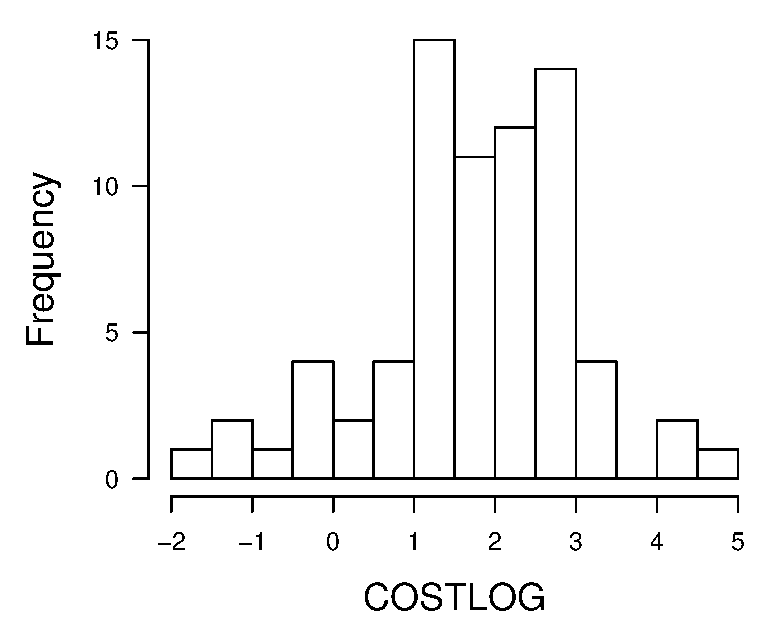
\includegraphics[width=0.4\textwidth]{Chapter6/F6HistCostLog.eps}
    \caption{\label{F6:HistCostLog} \small {Histogram of COSTLOG (the
    natural logarithm of FIRMCOST). The distribution of COSTLOG is
    less skewed than that of FIRMCOST.}}
  \end{center}
\end{figure}

\begin{figure}[htp]
  \begin{center}
   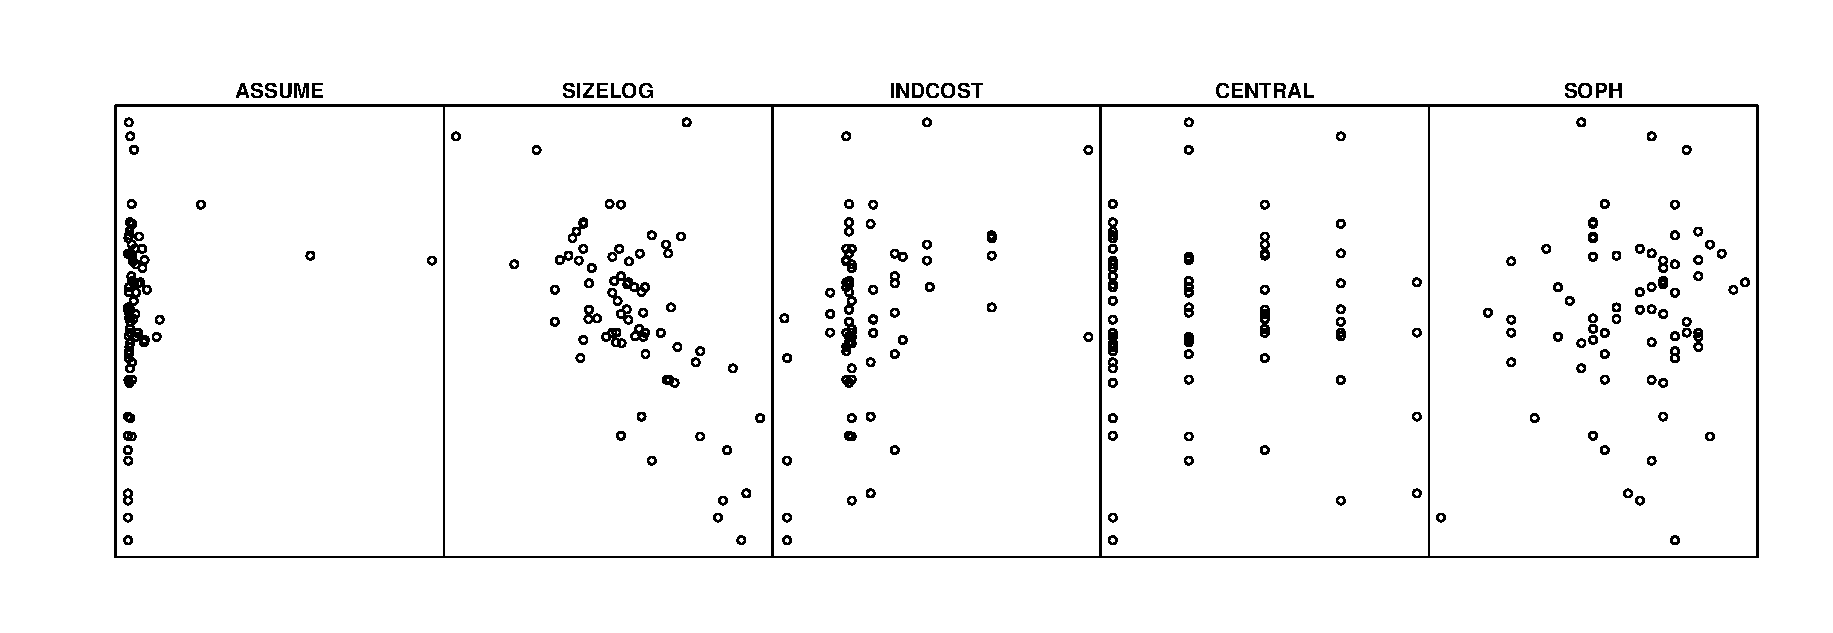
\includegraphics[width=1\textwidth]{Chapter6/F6CostLogPlots.eps}
    \caption{\label{F6:CostLogPlots}
    \small {Scatter plots of COSTLOG versus several explanatory variables.
    There is a negative relationship between COSTLOG and SIZELOG and
    a mild positive relationship between COSTLOG and INDCOST.}}
  \end{center}
\end{figure}

\bigskip

\subsubsection*{Some New Models}

Now, we explore the use of COSTLOG as the dependent variable. This
line of thought is based on the work in the previous subsection and
the plots of residuals from the preliminary regression fit. As a
first step, we fit a model with all explanatory variables. Thus,
this model is the same as the preliminary regression fit except
using COSTLOG in lieu of FIRMCOST as the dependent variable. This
model serves as a useful benchmark for our subsequent work. Table
\ref{T6:FirmRiskNew} summarizes the fit.


\begin{table}[h]
\scalefont{0.9} \caption{\label{T6:FirmRiskNew} Regression Results -
COSTLOG as Dependent Variable}
\begin{tabular}{l|rrr}
\hline
 &  & Standard &  \\
Variable & Coefficient & Error & $t$-statistic \\
\hline
INTERCEPT & 7.64 & 1.16 & 6.62 \\
ASSUME & -0.008 & 0.013 & -0.61 \\
CAP & 0.015 & 0.233 & 0.06 \\
SIZELOG & -0.787 & 0.117 & -6.75 \\
INDCOST & 1.90 & 0.503 & 3.79 \\
CENTRAL & -0.080 & 0.087 & -0.92 \\
SOPH & 0.002 & 0.021 & 0.12 \\
\hline
\end{tabular}
\scalefont{1.1111}  \end{table}

\noindent Here, $R_{a}^{2}=48\%$, \textit{F-}ratio $=12.1$ and
$s=0.882$. Figure \ref{F6:ResidLeverage2} shows that the
distribution of standardized residuals is less skewed than the
corresponding in Figure \ref{F6:ResidLeverage1}. The distribution of
leverages shows that there are still highly influential
observations. (As a matter of fact, the distribution of leverages
appear to be the same as in Figure \ref{F6:ResidLeverage1}. Why?)
Four of the six variables have \textit{t-}ratios less than one in
absolute value, suggesting that we continue our search for a better
model.

\begin{figure}[htp]
  \begin{center}
   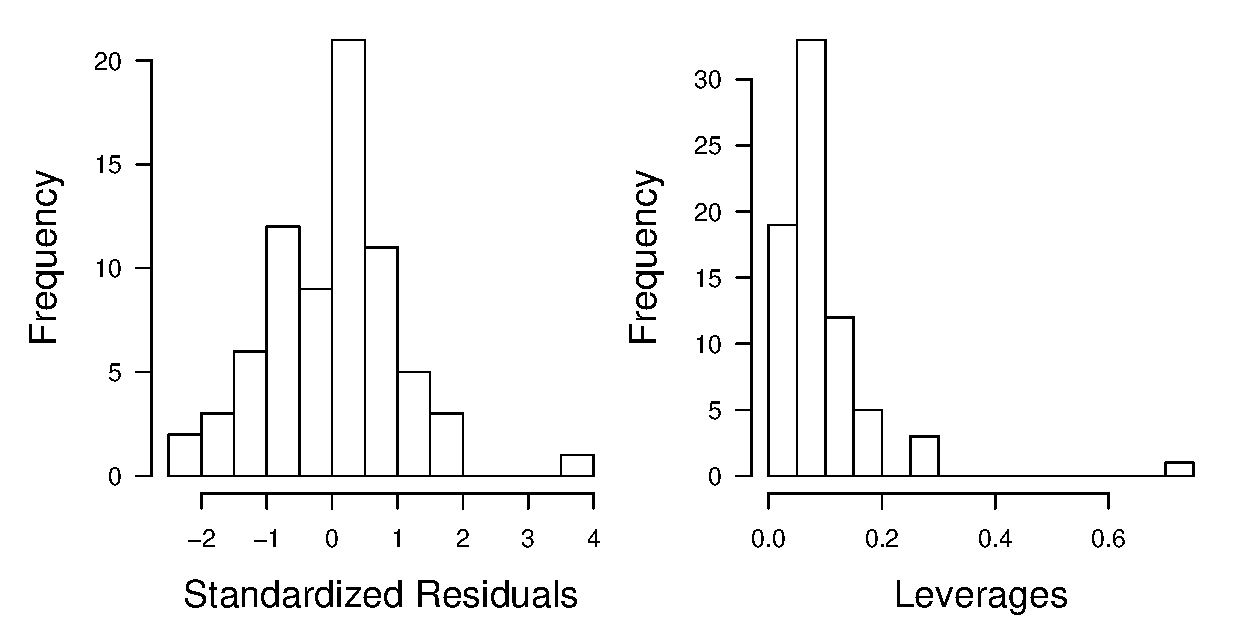
\includegraphics[width=0.6\textwidth]{Chapter6/F6ResidLeverage2.eps}
    \caption{\label{F6:ResidLeverage2} \small {Histograms of
    standardized residuals and leverages using COSTLOG as the
    dependent variable.}}
  \end{center}
\end{figure}

To continue the search, a stepwise regression was run (although the
output is not reproduced here). The output from this search
technique, as well as the fitted regression model above, suggests
using the variables SIZELOG and INDCOST to explain the dependent
variable COSTLOG.

A regression was run using SIZELOG and INDCOST as explanatory
variables. From Figure \ref{F6:ResidLeverage3}, we see that the size
and shape of the distribution of standardized residuals are similar
to that in Figure \ref{F6:ResidLeverage2}. The leverages are much
smaller, reflecting the elimination of several explanatory variables
from the model. Remember that the average leverage is $\bar{h}%
=(k+1)/n=3/73\approx 0.04$. Thus, we still have three points that exceed
three times the average and thus are considered high leverage points.


\begin{figure}[htp]
  \begin{center}
   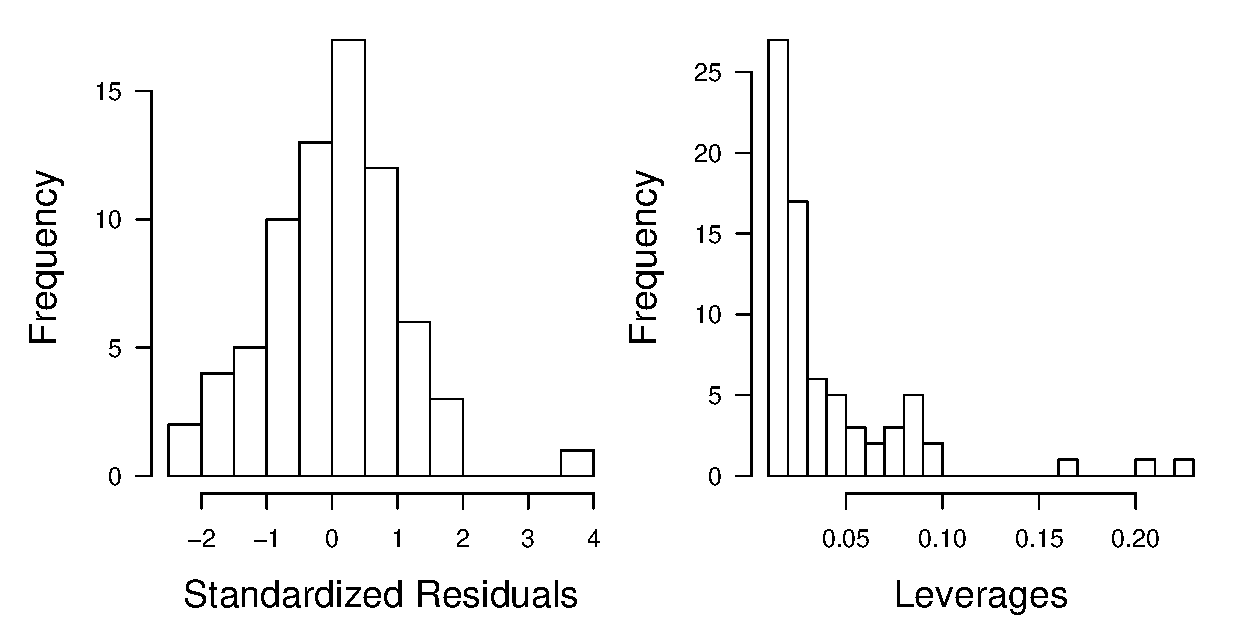
\includegraphics[width=0.6\textwidth]{Chapter6/F6ResidLeverage3.eps}
    \caption{\label{F6:ResidLeverage3} \small {Histograms of
    standardized residuals and leverages using SIZELOG and INDCOST
    as explanatory variables.}}
  \end{center}
\end{figure}


\begin{figure}[htp]
  \begin{center}
   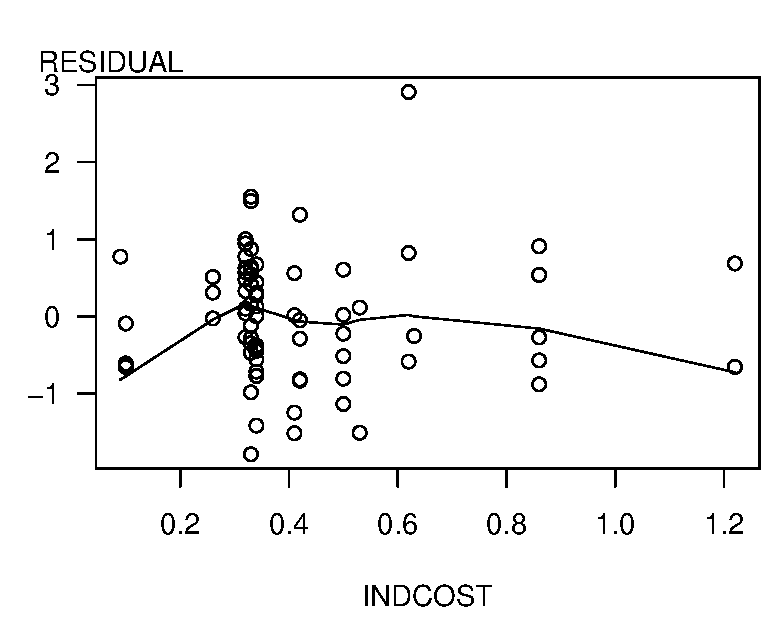
\includegraphics[width=0.6\textwidth]{Chapter6/F6SurveyQuad.eps}
    \caption{\label{F6:SurveyQuad} \small {Scatter plot of residuals versus INDCOST.
    The smooth fitted curve (using lowess) suggests a quadratic term in INDCOST.}}
  \end{center}
\end{figure}\index{plots!scatterplot smoothing!lowess}



Plots of residuals versus the explanatory variables reveal some mild
patterns. The scatter plot of residuals versus INDCOST, in Figure
\ref{F6:SurveyQuad}, displays a mild quadratic trend in INDCOST. To
see if this trend was important, the variable INDCOST was squared
and used as an explanatory variable in a regression model. The
results of this fit are in Table \ref{T6:FirmRiskQuad}.



\begin{table}[h]
\scalefont{0.9} \caption{\label{T6:FirmRiskQuad} Regression Results
with a Quadratic term in INDCOST}
\begin{tabular}{l|rrr}
\hline
 &  & Standard &  \\
Variable & Coefficient & Error & $t$-statistic \\
\hline
INTERCEPT & 6.35 & 0.953 & 6.67 \\
SIZELOG & -0.773 & 0.101 & -7.63\\
INDCOST & 6.26 & 1.61 & 3.89\\
INDCOST$^2$ & -3.58 & 1.27 & -2.83 \\

\hline
\end{tabular}
\scalefont{1.1111}  \end{table}

From the \textit{t-}ratio associated with (INDCOST)$^{2}$, we see
that the variable seems to be important. The sign is reasonable,
indicating that the rate of increase of COSTLOG decreases as INDCOST
increases. That is, the expected change in COSTLOG per unit change
of INDCOST is positive and decreases as INDCOST increases.

Further diagnostic checks of the model revealed no additional patterns.
Thus, from the data available, we can not affirm any of the four hypotheses
that were introduced in the Introduction subsection. This is not to say that
these variables are not important. We are simply stating that the natural
variability of the data was large enough to obscure any relationships that
might exist. We have established, however, the importance of the size of the
firm and the firm's industry risk.

Figure \ref{F6:SurveySummary} graphically summarizes the estimated
relationships among these variables. In particular, in lower right
hand panel, we see that for most of the firms in the sample,
FIRMCOST was relatively stable. However, for small firms, as
measured by SIZELOG, the industry risk, as measured by INDCOST, was
particularly important. For small firms, we see that the fitted
FIRMCOST increases as the variable INDCOST increases, with the rate
of increase leveling off. Although the model theoretically predicts
FIRMCOST to decrease with a large INDCOST $(>1.2)$, no small firms
were actually in this area of the data region.


\begin{figure}[htp]
  \begin{center}
   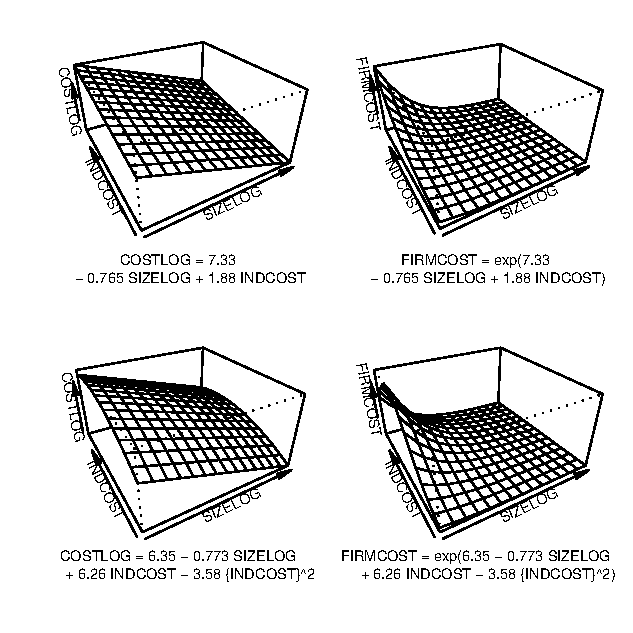
\includegraphics[width=0.8\textwidth]{Chapter6/F6SurveySummary.eps}
    \caption{\label{F6:SurveySummary} \small {Graph of four fitted
    models versus INDCOST and SIZELOG. }}
  \end{center}
\end{figure}


\section{Further Reading and References}

This chapter concludes our Part I, an introduction to linear
regression. To learn more about linear regression, in Section 1.7 we
gave references to alternative statistics books that introduce the
topic. You may also be interested in a more technical presentation,
such as the classic work by Seber (1977) or a more recent work by
Abraham and Ledolter (2006). For other approaches, texts such as
Wooldridge (2009) provide an econometrics perspective where the
emphasis is on introducing regression in the context of economic
theory. Alternatively, books such as Agresti and Finlay (2008) give
an introduction from a broader social science perspective.

There are many explanations of regression for readers with different
perspectives and levels of quantitative training; this provides
further evidence that this is an important topic for actuaries and
other financial risk managers to understand. The other way of
getting further insights into linear regression is to see it applied
in a time series context in Part II of this book or in extensions to
nonlinear modeling in Part III.

See Bollen (1989) for a classic introduction to structural equations
modeling.

\bigskip


\textbf{Chapter References}

\begin{multicols}{2}

\scalefont{0.9}

Abraham, Bova and Johannes Ledolter (2006). \textit{Introduction to
Regression Modeling.} Thomson Higher Education, Belmont, CA.

Agresti, Alan and Barbara Finlay (2008). \textit{Statistical Methods
for the Social Sciences, Fourth Edition}. Prentice Hall, Upper
Saddle, NJ.

Bollen, Kenneth A. (1989). \textit{Structural Equations with Latent
Variables}. New York: Wiley.

Box, George E. P. (1979). Robustness in the strategy of scientific
model building. In R. Launer and G. Wilderson (editors),
\textit{Robustness in Statistics}, pages 201-236, Academic Press,
New York.

Faraway, Julian J. (2005). \textit{Linear Models with R}. Chapman \&
Hall/CRC, Boca Raton, Florida.

Fienberg, S. E (1985). Insurance availability in Chicago. Chapter in
\textit{Data: A Collection of Problems from Many Fields for the
Student and Research Worker}. Editors D.F. Andrews and A. M.
Herzberg, Springer-Verlag, New York.

Goldberger, Arthur S. (1972).  Structural equation methods in the
social sciences.  \textit{Econometrica} 40, 979-1001.

Harrington, Scott E. and Greg Niehaus (1998). Race, redlining and
automobile insurance prices. \textit{Journal of Business} 71(3),
439-469.

Heckman, J. J. (1976). The common structure of statistical models of
truncation, sample selection and limited dependent variables, and a
simple estimator for such models. \textit{Ann. Econ. Soc. Meas}. 5,
475-492.

Little, R. J.  (1995). Modelling the drop-out mechanism in
repeated-measures studies. \textit{Journal of the American
Statistical Association} 90, 1112-1121.

Little, R. J. and Rubin, D. B. (1987).  \textit{Statistical Analysis
with Missing Data.}  John Wiley, New York.

Roberts, Harry V. (1990). Business and economic statistics (with
discussion). \textit{Statistical Science} 4, 372-402.

Rubin, D. R. (1976). Inference and missing data. \textit{Biometrika}
63, 581-592.

Schmit, Joan T. and K. Roth (1990). Cost effectiveness of risk
management practices. \textit{The Journal of Risk and Insurance} 57,
No. 3, pages 455-470.

Seber, G. A. F. (1977). \textit{Linear Regression Analysis.} John
Wiley \& Sons, New York.

Wachter, K. W.  and J. Trusell (1982). Estimating historical
heights. \textit{Journal of the American Statistical Association}
77, 279-301.

Wooldridge, Jeffrey (2009). \textit{Introductory Econometrics: A
Modern Approach, Fourth Edition.} South-Western Publishing, Mason,
Ohio.

\scalefont{1.1111}

\end{multicols}

\section{Exercises}

\scalefont{0.90}

\begin{exercises}

\empexjed{Chicago}\index{datasets!insurance redlining}

\item \textbf{Insurance Redlining.} Do insurance companies use race as a determining factor when making
insurance available? Fienberg (1985) gathered data from a report
issued by the U.S. Commission on Civil Rights about the number of
homeowners and residential fire insurance policies issued in Chicago
over the months of December 1977 through February 1978. Policies
issued were categorized as either part of the standard voluntary
market or the substandard, involuntary market. The involuntary
market consists of ``fair access to insurance requirements'' (FAIR)
plans; these are state insurance programs sometimes subsidized by
private companies. These plans provide insurance to people who would
otherwise be denied insurance on their property due to high-risk
problems. The main purpose is to understand the relationship between
insurance activity and the variable ``race,'' the percentage
minority. Data are available for $n=47$ zip codes in the Chicago
area. These data have also been analyzed by Faraway (2005).

To help control for the size of the expected loss, Fienberg also
gathered theft and fire data from Chicago's police and fire
departments. Another variable that gives some information about loss
size is the age of the house. The median income, from the Census
Bureau, gives indirect information on the size of the expected loss
as well as whether the applicant can afford insurance. Table
\ref{Ex:InsChicago} provides more details on these variables.


\begin{table}[h]
\caption{\label{Ex:InsChicago} \small Insurance Availability in
Chicago}
\begin{center}
\scalefont{0.8}
\begin{tabular}{l|l|r}
\hline
\bf Variable & \multicolumn{1}{c}{\bf Description} &\multicolumn{1}{|c}{\bf Mean} \\
\hline
row.names & Zip (postal) code \\
race & Racial composition in percent minority & 35.0\\
fire & Fires per 1,000 housing units & 12.3\\
theft & Thefts per 1,000 population & 32.4\\
age & Percent of housing units built in or before 1939 & 60.3\\
volact & New homeowner policies plus renewals, minus cancelations \\
&~~~and non-renewals per 100 housing units &6.53\\
involact & New FAIR plan policies and renewals per 100 housing units
& 0.615\\
income & Median family income & 10,696\\
\hline
\multicolumn{3}{c} {\textit{Source}: Fienberg (1985)} \\
\hline
\end{tabular}
\end{center}
\scalefont{1.25}
\end{table}


a. Produce summary statistics of all variables,  noting patterns of
skewness for each variable.

b. Create a scatter plot matrix of volact, involact and race.
Comment on the three pairwise relationships. Are the patterns
consistent with a hypothesis of racial discrimination?

c. To understand relationships among the variables, produce a table
of correlations.

d. Fit a linear model using volact as the dependent variable and
race, fire theft, age and income as explanatory variables.

d(i). Comment on the sign and statistical significance of the
coefficient associated with race.

d(ii). Two zip codes turn out to have high leverage. Repeat your
analysis after deleting these two observations. Has the significance
of the race variable changed? What about the other explanatory
variables?

e. Repeat the analysis in part (d) using involact as the dependent
variable.

f. Define proportion to be involact/(volact+involact). Repeat the
analysis in part (d) using proportion as the dependent variable.

g. The same two zip codes have high leverage in parts (d), (e) and
(f). Why is this so?

h. This analysis is done at the zip code level, not the individual
level. As emphasized by Harrington and Niehaus (1998), this
introduces substantial potential omitted variable bias. What
variables have been omitted from the analysis that you think might
affect homeowners insurance availability and race?

i. Fienberg notes that proximity of one zip code to another may
affect the dependence of observations. Describe how you might
incorporate spatial relations into a regression analysis.


\item \textbf{Gender Equity in Faculty Pay.} The University of Wisconsin at Madison completed a study entitled
``Gender Equity Study of Faculty Pay,'' dated June 5, 1992. The main
purpose of the study was to determine whether women are treated
unfairly in salary determinations at a major research university in
the U.S. To this end, the committee that issued the report studied
1990 salaries of 1,898 faculty members in the university. It is
well-known that men are paid more than women. In fact, the mean 1990
salary for the 1,528 male faculty members is \$54,478, which is 28\%
higher than the mean 1990 salary for female faculty members, which
is \$43,315. However, it is argued that male faculty members are in
general more senior (average years of experience is 18.8 years) than
female faculty members (average years of experience is 11.9 years),
and thus deserved higher pay. When comparing salaries of full
professors (thus controlling for years of experience), male faculty
members earned about 13\% more than their female counterparts. Even
so, it is generally agreed that fields in demand must offer higher
salaries in order to maintain a world-class faculty. For example,
salaries in engineering are higher than salaries in humanities
simply because faculty in engineering have many more employment
opportunities outside of academia than faculty in humanities. Thus,
when considering salaries, one must also control for department.

To control for these variables, a faculty study reports a regression
analysis using the logarithm of salary as the dependent variable.
The explanatory variables included information on race, gender, rank
(either assistant professor/instructor, associate professor or full
professor), several measures of years of experience, 98 different
categories of departments and a measure of salary differential by
department. There were 109 explanatory variables in all (including
97 departmental binary variables), of which 12 were non-departmental
variables. Table \ref{Ex:FacultyPay} reports variable definitions,
parameter estimates and $t$-ratios for the 12 non-departmental
variables. The ANOVA Table \ref{Ex:FacultyPayANOVA} summarizes the
regression fit.


\begin{table}[h]
\caption{\label{Ex:FacultyPay} \small Non-Departmental Variables and
Parameter Estimates}
\begin{center}
\scalefont{0.8}
\begin{tabular}{llrr}
\hline
Explanatory  & Variable Description & Parameter& $t$-ratio \\
Variable &  &  Estimate &  \\
\hline INTERCEPT &            &    10.746 &      261.1 \\
    GENDER & = 1 if male, 0 otherwise &     0.016 &       1.86 \\
      RACE & = 1 if white, 0 otherwise &    -0.029 &      -2.44 \\
      FULL & = 1 if a full professor, 0 otherwise &     0.186 &      16.42 \\
 ASSISTANT & = 1 if an assistant professor, 0 otherwise &    -0.205 &     -15.93 \\
    ANYDOC & = 1 if has a terminal degree such as a Ph.D. &     0.022 &       1.11 \\
   COHORT1 & = 1 if hired before 1969, 0 otherwise &    -0.102 &      -4.84 \\
   COHORT2 & = 1 if hired 1969-1985, 0 otherwise &    -0.046 &      -3.48 \\
 FULLYEARS & Number of years as a full professor at UW &     0.012 &      12.84 \\
ASSOCYEARS & Number of years as an associate professor at UW &    -0.012 &      -8.65 \\
ASSISYEARS & Number of years as an assistant professor &    &     \\
    & ~~ or an instructor at UW &     0.002 &        0.91 \\
    DIFYRS & Number of years since receiving a terminal degree&      &        \\
   & ~~ before arriving to UW &     0.004 &       4.46 \\
 MRKTRATIO & Natural logarithm of a ``market ratio''  &      &        \\
&  ~~- defined as the ratio of the average salary  &      &       \\
 &  ~~~~at peer institutions for a given discipline and rank &     0.665 &       7.64 \\
\hline
\end{tabular}

\noindent \textit{Source:} ``Gender Equity Study of Faculty Pay,''
June 5, 1992, The University of Wisconsin at Madison.
\end{center}
\scalefont{1.25}
\end{table}


\begin{table}[h]
\caption{\label{Ex:FacultyPayANOVA} \small Faculty Pay ANOVA Table}
\begin{center}
\scalefont{0.8}
\begin{tabular}{l|rrrr}
\hline Source & Sum of Squares & $df$ & Mean Square & $F$-ratio\\
\hline
Regression & 114.048 & 109 & 1.0463 & 62.943\\
Error & 29.739 & 1789 & 0.0166 &\\
Total & 143.788 & 1898 &  &\\ \hline
\end{tabular}
\end{center}
\scalefont{1.25}
\end{table}

a. Suppose that a female faculty member in the chemistry department
feels that her salary is below what it should be. Briefly describe
how this study can be used as a basis for performance evaluation.

b. Based on this study, do you think that salaries of women are
significantly lower than men?

b(i). Cite statistical arguments supporting the fact that men are
not paid significantly more than women.

b(ii). Cite statistical arguments supporting the fact that men are
paid significantly more than women.

b(iii). Suppose that you decide that women are paid less than men.
Based on this study, how much would you raise female faculty members
salaries to be on par with their male counterparts?


\end{exercises}
\scalefont{1.1111}

\section{Technical Supplements for Chapter 6}
\scalefont{0.9}


\subsection{Effects of Model Misspecification}

\textbf{Notation.} Partition the matrix of explanatory variables
$\mathbf{X}$ into two submatrices, each having $n$ rows, so that
$\mathbf{X}=(\mathbf{X} _{1} : \mathbf{X}_{2})$. For convenience,
assume that $\mathbf{X}_{1}$ is an $ n\times p$ matrix. Similarly,
partition the vector of parameters $\boldsymbol \beta =\left(
\boldsymbol \beta _{1}^{\prime }, \boldsymbol \beta _{2}^{\prime
}\right) ^{\prime }$ such that $\mathbf{X \boldsymbol \beta
}=\mathbf{X}_{1} \boldsymbol \beta_{1}+ \mathbf{X}_{2} \boldsymbol
\beta_{2}$. We compare the full, or ``long,'' model
\begin{center}
\[
\mathbf{y}=\mathbf{X \boldsymbol \beta }+\boldsymbol \varepsilon = \mathbf{X}_{1} \boldsymbol \beta_{1}+%
\mathbf{X}_{2} \boldsymbol \beta_{2}+\boldsymbol \varepsilon
\]
\end{center}
to the reduced, or ``short,'' model
\begin{center}
\[
\mathbf{y}=\mathbf{X}_{1} \boldsymbol \beta_{1}+\boldsymbol
\varepsilon.
\]
\end{center}
This simply generalizes the set-up earlier to allow for omitting
several variables.

\textbf{Effect of Underfitting.} Suppose that the true
representation is the long model but we mistakenly run the short
model. Our parameter estimates
when running the short model are given by $\mathbf{b}_{1}=\mathbf{(X}%
_{1}^{\prime }\mathbf{X}_{1}\mathbf{)}^{-1}\mathbf{X}_{1}^{\prime
}\mathbf{y} $. These estimates are biased because
\begin{center}
\begin{eqnarray*}
\text{Bias} &=&\text{E }\mathbf{b}_{1}-\boldsymbol \beta_{1}
=\text{E}\mathbf{(X%
}_{1}^{\prime }\mathbf{X}_{1}\mathbf{)}^{-1}\mathbf{X}_{1}^{\prime }\mathbf{y%
}-\boldsymbol \beta_{1}
=\mathbf{(X}_{1}^{\prime }\mathbf{X}_{1}\mathbf{)}^{-1}%
\mathbf{X}_{1}^{\prime }\text{E }\mathbf{y}-\boldsymbol \beta_{1} \\
&=&\mathbf{(X}_{1}^{\prime }\mathbf{X}_{1}\mathbf{)}^{-1}\mathbf{X}%
_{1}^{\prime }\left( \mathbf{X}_{1}\boldsymbol
\beta_{1}+\mathbf{X}_{2}\boldsymbol \beta_{2}\right)
- \boldsymbol \beta_{1}=\mathbf{(X}_{1}^{\prime }\mathbf{X}%
_{1}\mathbf{)}^{-1}\mathbf{X}_{1}^{\prime }\mathbf{X}_{2}\boldsymbol \beta_{2}=%
\mathbf{A \boldsymbol \beta }_{2}.
\end{eqnarray*}
\end{center}
Here, $\mathbf{A}=\mathbf{(X}_{1}^{\prime }\mathbf{X}_{1}\mathbf{)}^{-1}%
\mathbf{X}_{1}^{\prime }\mathbf{X}_{2}$ is called the
\textit{alias}, or
bias, matrix. When running the short model, the estimated variance is $%
s_{1}^{2}=(\mathbf{y}^{\prime }\mathbf{y}-\mathbf{b}_{1}^{\prime }\mathbf{X}%
_{1}^{\prime }\mathbf{y})/(n-p)$. It can be shown that
\begin{equation}\label{E5:AliasBias}
\text{E }s_{1}^{2}=\sigma ^{2}+(n-p)^{-1}\boldsymbol
\beta_{2}^{\prime }\left(
\mathbf{X}_{2}^{\prime }\mathbf{X}_{2}-\mathbf{X}_{2}^{\prime }\mathbf{X}_{1}%
\mathbf{(X}_{1}^{\prime
}\mathbf{X}_{1}\mathbf{)}^{-1}\mathbf{X}_{1}^{\prime
}\mathbf{X}_{2}\right) \boldsymbol \beta_{2}.
\end{equation}
Thus, $s_{1}^{2}$ is an ``overbiased'' estimate of $\sigma ^{2}$.

Let $\mathbf{x}_{1i}^{\prime }$ and $\mathbf{x}_{2i}^{\prime }$ be
the $i$th rows of $\mathbf{X}_{1}$ and $\mathbf{X}_{2}$,
respectively. Using
the fitted short model, the $i$th fitted value is $\hat{y}_{1i}=\mathbf{x}%
_{1i}^{\prime }\mathbf{b}_{1}$. The true $i$th expected response is E $\hat{y%
}_{1i}=\mathbf{x}_{1i}^{\prime } \boldsymbol \beta_{1}+$
$\mathbf{x}_{2i}^{\prime } \boldsymbol \beta_{2}$. Thus, the bias of
the $i$th fitted value is

\begin{center}
\begin{eqnarray*}
\text{Bias}(\hat{y}_{1i}) &=&\text{E }\hat{y}_{1i}-\text{E }y_{i}=\mathbf{x}%
_{1i}^{\prime }\text{E }\mathbf{b}_{1}-\left( \mathbf{x}_{1i}^{\prime }%
\boldsymbol \beta_{1}+\mathbf{x}_{2i}^{\prime } \boldsymbol \beta_{2}\right)  \\
&=&\mathbf{x}_{1i}^{\prime }(\boldsymbol \beta_{1}+\mathbf{A \boldsymbol \beta }%
_{2})-\left( \mathbf{x}_{1i}^{\prime }\boldsymbol \beta_{1}+\mathbf{x}%
_{2i}^{\prime }\boldsymbol \beta_{2}\right) =(\mathbf{x}_{1i}^{\prime }\mathbf{%
A}-\mathbf{x}_{2i}^{\prime })\boldsymbol \beta_{2}.
\end{eqnarray*}
\end{center}

Using this and equation (\ref{E5:AliasBias}), straightforward
algebra show that
\begin{equation}\label{E5:SumBias}
\text{E }s_{1}^{2}=\sigma ^{2}+(n-p)^{-1}\sum_{i=1}^{n}(\text{Bias}(\hat{y}%
_{1i}))^{2}.
\end{equation}

\textbf{Effect of Overfitting.} Now suppose that the true
representation is the short model but we mistakenly use the large
model. With the alias matrix
$\mathbf{A}=\mathbf{(X}_{1}^{\prime }\mathbf{X}_{1}%
\mathbf{)}^{-1}\mathbf{X}_{1}^{\prime }\mathbf{X}_{2},$ we can \textit{%
reparameterize} the long model
\begin{center}
\[
\mathbf{y}=\mathbf{X}_{1}\boldsymbol
\beta_{1}+\mathbf{X}_{2}\boldsymbol \beta_{2} + \boldsymbol
\varepsilon
=\mathbf{X}_{1}\left( \boldsymbol \beta_{1}+\mathbf{A \boldsymbol \beta }%
_{2}\right) +\mathbf{E}_{1}\boldsymbol \beta_{2} + \boldsymbol
\varepsilon = \mathbf{X}_{1}%
\boldsymbol \alpha_{1}+\mathbf{E}_{1}\boldsymbol \beta_{2} +
\boldsymbol \varepsilon
\]
\end{center}
where
$\mathbf{E}_{1}=\mathbf{X}_{2}\mathbf{-X}_{1}\mathbf{A}$\textbf{\
}and $\boldsymbol \alpha_{1}=\boldsymbol \beta_{1}+\mathbf{A
\boldsymbol \beta}_{2}$. The advantage of this new parameterization
is that $\mathbf{X}_{1}$ is
orthogonal to $\mathbf{E}_{1}$ because $\mathbf{X}_{1}^{\prime }\mathbf{E}%
_{1}=\mathbf{X}_{1}^{\prime }(\mathbf{X}_{2}-\mathbf{X}_{1}\mathbf{A})=%
\mathbf{0}$. With $\mathbf{X}^{\ast }=(\mathbf{X}%
_{1}: \mathbf{E}_{1})$ and $\boldsymbol \alpha =(\boldsymbol \alpha_{1}^{\prime }%
\boldsymbol \beta_{1}^{\prime })^{\prime }$, the vector of least
squares estimates is
\begin{center}
\begin{eqnarray*}
\mathbf{a} &=&%
\begin{bmatrix}
\mathbf{a}_{1} \\
\mathbf{b}_{1}%
\end{bmatrix}%
=\left( \mathbf{X}^{\ast \prime }\mathbf{X}^{\ast }\right) ^{-1}\mathbf{X}%
^{\ast \prime }\mathbf{y} \\
&=&%
\begin{bmatrix}
\mathbf{(X}_{1}^{\prime }\mathbf{X}_{1}\mathbf{)}^{-1} & 0 \\
0 & \mathbf{(E}_{1}^{\prime }\mathbf{E}_{1}\mathbf{)}^{-1}%
\end{bmatrix}%
\begin{bmatrix}
\mathbf{X}_{1}^{\prime }\mathbf{y} \\
\mathbf{E}_{1}^{\prime }\mathbf{y}%
\end{bmatrix}%
=%
\begin{bmatrix}
\mathbf{(X}_{1}^{\prime
}\mathbf{X}_{1}\mathbf{)}^{-1}\mathbf{X}_{1}^{\prime
}\mathbf{y} \\
\mathbf{(E}_{1}^{\prime
}\mathbf{E}_{1}\mathbf{)}^{-1}\mathbf{E}_{1}^{\prime
}\mathbf{y}%
\end{bmatrix}%
.
\end{eqnarray*}
\end{center}

From the true (short) model, E $\mathbf{y}=\mathbf{X}_{1}\boldsymbol \beta_{1}$%
, we have that E $\mathbf{b}_{2}=(\mathbf{E}_{1}^{\prime }\mathbf{E}%
_{1})^{-1}\mathbf{E}_{1}^{\prime }$E $\mathbf{y}=(\mathbf{E}_{1}^{\prime }%
\mathbf{E}_{1})^{-1}\mathbf{E}_{1}^{\prime }$E
$(\mathbf{X}_{1}\mathbf{\beta
}_{1})=\mathbf{0}$, because $\mathbf{X}_{1}^{\prime }\mathbf{E}_{1}=\mathbf{%
0.}$  The least squares estimate of $\boldsymbol \beta_{1}$ is $\mathbf{b}_{1}=\mathbf{a%
}_{1}-\mathbf{Ab}_{2}$. Because E $\mathbf{a}_{1}=$
$\mathbf{(X}_{1}^{\prime
}\mathbf{X}_{1}\mathbf{)}^{-1}\mathbf{X}_{1}^{\prime }$E
$\mathbf{y}=\boldsymbol \beta_{1}$ under the short model, we have E $\mathbf{b}_{1}=$ E $\mathbf{a}%
_{1}-\mathbf{A}$E $\mathbf{b}_{2}=\boldsymbol
\beta_{1}-\mathbf{0}=\boldsymbol \beta_{1}$. Thus, even though we mistakenly run the long model, $\mathbf{b}%
_{1}$ is still an unbiased estimator of $\boldsymbol \beta_{1}$ and $\mathbf{b}%
_{2}$ is an unbiased estimator of $\mathbf{0}$. Thus, there is no
bias in
the $i$th fitted value because E $\hat{y}_{i}=$ E $(\mathbf{x}_{1i}^{\prime }%
\mathbf{b}_{1}+\mathbf{x}_{2i}^{\prime }\mathbf{b}_{2})=\mathbf{x}%
_{1i}^{\prime }\boldsymbol \beta_{1}=$ E $y_{i}$.

$\mathbf{C}_{\mathbf{p}}$\textbf{\ Statistic.} Suppose initially
that the true representation is the long model but we mistakenly use
the short model.
The $i$th fitted value is $\hat{y}_{1i}=$ $\mathbf{x}_{1i}^{\prime }\mathbf{b%
}_{1}$ that has mean square error
\begin{center}
\[
\text{MSE }\hat{y}_{1i}=\text{E}(\hat{y}_{1i}-\text{E }\hat{y}_{1i})^{2}=%
\text{Var }\hat{y}_{1i}+\left( \text{Bias }\hat{y}_{1i}\right) ^{2}.
\]
\end{center}
For the first part, we have that Var $\hat{y}_{1i}=$ Var  $\left( \mathbf{x}%
_{1i}^{\prime }\mathbf{b}_{1}\right) =$ Var $\left( \mathbf{x}_{1i}^{\prime }%
\mathbf{(X}_{1}^{\prime
}\mathbf{X}_{1}\mathbf{)}^{-1}\mathbf{X}_{1}^{\prime
}\mathbf{y}\right) =\sigma ^{2}\mathbf{x}_{1i}\mathbf{(X}_{1}^{\prime }%
\mathbf{X}_{1}\mathbf{)}^{-1}\mathbf{x}_{1i}^{\prime }$. We can think of $%
\mathbf{x}_{1i}\mathbf{(X}_{1}^{\prime }\mathbf{X}_{1}\mathbf{)}^{-1}\mathbf{%
x}_{1i}^{\prime }$ as the $i$th leverage, as in equation
(\ref{E5:Leverage}). Thus, $\sum_{i=1}^{n}\mathbf{x}_{1i}\mathbf{%
(X}_{1}^{\prime
}\mathbf{X}_{1}\mathbf{)}^{-1}\mathbf{x}_{1i}^{\prime }=p$, the
number of columns of $\mathbf{X}_{1}$. With this, we can define the
\textit{standardized total error}

\begin{center}
\begin{eqnarray*}
\frac{\sum_{i=1}^{n}\text{MSE }\hat{y}_{1i}}{\sigma ^{2}} &=&\frac{%
\sum_{i=1}^{n}\left( \text{Var }\hat{y}_{1i}+\left( \text{Bias }\hat{y}%
_{1i}\right) ^{2}\right) }{\sigma ^{2}} \\
&=&\frac{\sigma ^{2}\sum_{i=1}^{n}\left( \mathbf{x}_{1i}\mathbf{(X}%
_{1}^{\prime }\mathbf{X}_{1}\mathbf{)}^{-1}\mathbf{x}_{1i}^{\prime
}+\left( \text{Bias }\hat{y}_{1i}\right) ^{2}\right) }{\sigma
^{2}}=p+\sigma ^{-2}\sum_{i=1}^{n}\left( \text{Bias
}\hat{y}_{1i}\right) ^{2}.
\end{eqnarray*}
\end{center}

Now, if $\sigma ^{2}$ is known, from equation (\ref{E5:SumBias}), an
unbiased estimate of the standardized total error is $
p+(n-p)(s_{1}^{2}-\sigma ^{2})/\sigma ^{2}.$ Because $\sigma ^{2}$
is unknown, it must be estimated. If we are not sure whether the
long or short model is the appropriate representation, a
conservative choice is to use $s^{2}$ from the long, or full, model.
Even if the short model is the true model, $s^{2}$ from the long
model is still an unbiased estimate of $\sigma ^{2}$. Thus, we
define

\begin{center}
\[
C_{p}=p+(n-p)(s_{1}^{2}-s^{2})/s^{2.}
\]
\end{center}

If the short model is correct, then E $s_{1}^{2}=$ E $s^{2}=\sigma
^{2}$ and E $C_{p}\approx p$. If the long model is true, then E
$s_{1}^{2}>\sigma ^{2}$ and E $C_{p}>p$.

\scalefont{1.1111}
